\documentclass[12pt,a4paper,twoside,open=right,bibliography=totoc,BCOR=10mm]{scrreprt}
\usepackage[utf8]{inputenc}
\usepackage[english,german]{babel}

\usepackage[T1]{fontenc} % Wichtig für alles was mehr als ASCII verwendet
\usepackage{csquotes} % Schöne Anführungsstriche mit \enquote{Text}
\usepackage{amsmath} % Bessere und schönere mathematische Formeln
\usepackage{mathtools} % Noch schönerere mathematische Formeln
\usepackage{amstext} % \text{} Macro in mathematischen Formeln
\usepackage{amsfonts} % Erweiterte Zeichensätze für mathematische Formeln
\usepackage{amssymb} % Spezielle mathematische Symbole.
\usepackage{array} % Matrizen in mathematischen Formeln
\usepackage{textcomp} % Für textmu und textohm etc. um im Fließtext keine Mathematik 
\usepackage{textalpha} % Damit können griechische Zeichen direkt im Text verwendet werden (siehe zeichen.txt)
\usepackage{paralist} % Für compactitem und compactenum
\usepackage{xstring} % Für IF in Titelseite
\usepackage{bm}
\usepackage{float}

\usepackage[version=3]{mhchem} % Für Chemische Formeln
\usepackage{braket} % Für das quantenmechanische Bra-Ket

\usepackage{geometry} % Seitenränder und Seiteneigenschaften setzen
%\usepackage[showframe]{geometry} % Anzeigen der Seitenränder, nützlich für debugging. http://ctan.org/pkg/geometry

\usepackage[bottom]{footmisc} % Zwingt Fußnoten an das Ende der Seite
\usepackage[pdftex]{hyperref} % Links richtig anzeigen. Sowohl innerhalb des Dokuments (Fußzeilen, Formeln), als auch ins Internet

\usepackage[ % Biblatex für die Zitate und Referenzen
	backend=biber,
	hyperref=true,
	sorting=none
		]{biblatex}

\usepackage{xkeyval} % Erlaubt "Variablen" zu definieren, wird für Titelseite gebraucht
\usepackage{graphicx} % Wichtig für das Einbinden von Grafiken
\usepackage{caption}
\usepackage{subcaption} % Einbinden von mehreren Grafiken in einer figure

\usepackage{dirtree} % Erlaubt das erstellen von Dateibäumen
%\dirtreecomment{Text} erstellt einen Kommentar zu dem Verzeichnis bzw. der Datei
\newcommand{\dirtreecomment}[1]{\dotfill{} \begin{minipage}[t]{0.5\textwidth}#1\end{minipage}}

\usepackage{fancyvrb} % Mehr Optionen für Verbatim
\usepackage{listings} % Zur Darstellung von Programmcode
\usepackage{pdflscape} % Querformat Seiten

\newcommand{\writeIn}[1]{\usepackage[#1]{babel}} % Definiert einen neuen Befehl um die Sprache des Dokuments zu setzen

\usepackage[usenames,dvipsnames]{color} % Farben für den todo Befehl
\newcommand{\todo}[1]{{\color{Cerulean}(TODO: #1)}} % Einfach \todo{Text} verwenden!

\newcommand{\blankpage}{ \newpage \thispagestyle{empty} \mbox{} \newpage }

\usepackage{glossaries}
\usepackage{parskip}
\usepackage[ruled,linesnumbered,algochapter]{algorithm2e} % Enables the writing of pseudo code.

\DeclareMathOperator{\arctantwo}{arctan2}


\hypersetup{
	pdfauthor={Andreas Stefl, BSc},
	pdftitle={Particle filter for online calibration of three axis magnetometers in smartphones},
	pdfsubject={Master thesis physics},
	pdfkeywords={},
	pdfdisplaydoctitle=true,
	colorlinks=false, % for printing "false"!
}

\addbibresource{references.bib}

\newacronym{ips}{IPS}{Indoor Positioning System}
\newacronym{gnss}{GNSS}{Global Navigation Satellite Systems}
\newacronym{gps}{GPS}{Global Positioning System}
\newacronym{imu}{IMU}{Inertial Measurement Unit}
\newacronym{pdr}{PDR}{Pedestrian Dead Reckoning}
\newacronym{mems}{MEMS}{Microelectromechanical Systems}

\newacronym{sis}{SIS}{Sequential Importance Sampling}
\newacronym{mc}{MC}{Monte Carlo}
\newacronym{mcmc}{MCMC}{Markov Chain Monte Carlo}
\newacronym{smc}{SMC}{Sequential Monte Carlo}
\newacronym{lqe}{LQE}{Linear Quadratic Estimation}
\newacronym{ls}{LS}{Least Squares}
\newacronym{rls}{RLS}{Recursive Least Squares}
\newacronym{mle}{MLE}{Maximum Likelihood Estimator}

\newacronym{os}{OS}{Operating System}
\newacronym{cpu}{CPU}{Central Processing Unit}
\newacronym{gpu}{GPU}{Graphics Processing Unit}
\newacronym{ram}{RAM}{Random Access Memory}
\newacronym{api}{API}{Application Programming Interface}
\newacronym{jni}{JNI}{Java Native Interface}

\newacronym{squid}{SQUID}{Superconducting Quantum Interference Device}

\makeglossaries

\begin{document}
\pagenumbering{gobble}

\selectlanguage{german}
\newgeometry{bottom=2cm, top=2cm, left=3cm, right=2cm}
\begin{titlepage}


\begin{tabular}{ >{\centering}p{9cm} >{\centering}p{7cm} }
	\space & {\line(1,0){120}\\Unterschrift Betreuer}
\end{tabular}

\begin{center}

% Upper part of the page
\begin{figure}[h]
	\centering
	\includegraphics[width=0.5\textwidth]{figures/TU_Wien_Logo.pdf}
	 %Logo gracefully taken from http://www.tuwien.ac.at/dle/pr/publishing_web_print/corporate_design/tu_logo/
\end{figure}

\vspace{\stretch{1}}
\begin{LARGE}

\par\noindent
DIPLOMARBEIT

\vspace{\stretch{1.6}}

\textbf{Particle Filter für automatische Laufzeit-Kalibrierung des 3-Achsen-Magnetometers in Smartphones} \\

\end{LARGE}

\vspace{\stretch{1.6}}
\begin{large}
ausgeführt am Institut für Angewandte Physik (IAP) \\
der Technischen Universität Wien

\vspace{\stretch{0.5}}

unter der Anleitung von \\
\textbf{Ao.Univ.Prof. Dipl.-Ing. Dr.techn. Martin Gröschl}

\vspace{\stretch{0.5}}

und Mitbetreuung von \\
\textbf{Dipl.-Ing. Dr.-Ing. Paolo Fogliaroni} \\
Esri R\&D Center Vienna

\vspace{\stretch{1}}

durch \\

\vspace{\stretch{0.3}}

\textbf{Andreas Stefl, BSc} \\

\vspace{\stretch{2}}

\begin{tabular}{ >{\centering}p{7cm} >{\centering}p{7cm} }
\centering
Wien, \today & \line(1,0){120}\\Unterschrift Student
\end{tabular}
\end{large}

\end{center}
\end{titlepage}
\restoregeometry

\selectlanguage{english}

\makeatletter
\define@cmdkey{ThesisTUWienPhysicsTitlePage}{author}[Max Mustermann]{}
\define@cmdkey{ThesisTUWienPhysicsTitlePage}{title}[Titel]{}
\define@cmdkey{ThesisTUWienPhysicsTitlePage}{institute}[Institut]{}
\define@cmdkey{ThesisTUWienPhysicsTitlePage}{prof}[Professor]{}
\define@cmdkey{ThesisTUWienPhysicsTitlePage}{address}[Adresse]{}
\define@cmdkey{ThesisTUWienPhysicsTitlePage}{type}[Typ der Arbeit]{}
\newcommand{\ThesisTUWienPhysicsTitlePage}[1]{\setkeys{ThesisTUWienPhysicsTitlePage}{#1}}

\setkeys{ThesisTUWienPhysicsTitlePage}{
	author=Max Mustermann,
	title=Titel,
	institute=Institut,
	prof=Professor,
	address=Adresse des Autors,
	type=bacc
}{}

\newcommand*{\titlePageTUWienPhysik}{
	\begingroup % Create the command for including the title page in the document
	\newgeometry{bottom=2cm, top=2cm, left=3cm, right=2cm}
	\begin{titlepage}
	
	
	\begin{tabular}{ >{\centering}p{9cm} >{\centering}p{7cm} }
		\space & {\line(1,0){120}\\Signature of Advisor}
	\end{tabular}
	
	\begin{center}

	% Upper part of the page
	\begin{figure}[h]
		\centering
		\includegraphics[width=0.5\textwidth]{figures/TU_Wien_Logo.pdf}
		% Logo gracefully taken from http://www.tuwien.ac.at/dle/pr/publishing_web_print/corporate_design/tu_logo/
	\end{figure}
	
	\vspace{\stretch{1}}
	\begin{LARGE}

	\par\noindent
	 \IfStrEqCase{\cmdKV@ThesisTUWienPhysicsTitlePage@type}{
	  {sem}{SEMINARARBEIT}
	  {bacc}{BACHELORARBEIT}
	  {proj}{PROJEKTARBEIT}
	  {mast}{DIPLOMARBEIT}
	  {dipl}{DIPLOMARBEIT}
	  {diss}{DISSERTATION}
	  }[\cmdKV@ThesisTUWienPhysicsTitlePage@type]

	\vspace{\stretch{1.8}}

	\textbf{\cmdKV@ThesisTUWienPhysicsTitlePage@title} \\

	\end{LARGE}
	
	\vspace{\stretch{1.8}}
	\begin{large}
	at \cmdKV@ThesisTUWienPhysicsTitlePage@institute \\
	TU Wien
	
	\vspace{\stretch{0.5}}
	
	Supervisor \\
	\textbf{\cmdKV@ThesisTUWienPhysicsTitlePage@prof}
	
	\vspace{\stretch{1}}
	
	by \\
	
	\vspace{\stretch{0.3}}
	
	\textbf{\cmdKV@ThesisTUWienPhysicsTitlePage@author} \\
	
	\vspace{\stretch{0.3}}
	
	\cmdKV@ThesisTUWienPhysicsTitlePage@address \\
	
	\vspace{\stretch{2}}
	
	\begin{tabular}{ >{\centering}p{7cm} >{\centering}p{7cm} }
	\centering
	\today & \line(1,0){120}\\Signature of Author
	\end{tabular}
	\end{large}
	
	\end{center}
	\end{titlepage}
	\restoregeometry
	\endgroup
}
\makeatother


\chapter*{Acknowledgements}
\addcontentsline{toc}{chapter}{Acknowledgements}
\label{ch:acknowledgements}
I wish to express my sincere gratitude to my supervisor Ao.Univ.Prof. Dipl.-Ing. Dr.techn. Martin Gröschl, my employer Esri R\&D Center Vienna and my manager and friend Thomas Taschauer. Without them, this thesis would not have been possible.

I want to thank my co-supervisor Dipl.-Ing. Dr.-Ing. Paolo Fogliaroni for proofreading my work and providing valuable feedback.

Further, I would like to thank my family and friends for supporting me under all circumstances.

Last but not least, I want to thank my girlfriend Samira for always supporting and encouraging me throughout the whole thesis.


\selectlanguage{german}
\chapter*{Kurzfassung}
\addcontentsline{toc}{chapter}{Kurzfassung}
\label{ch:kurzfassung}
Heutige Smartphones kommen im Normalfall mit einem eingebauten Magnetometer, welcher dazu benutzt werden kann die horizontale Orientierung zu bestimmen, wie bei einem Kompass. Das Smartphone besteht jedoch selbst aus magnetischen Materialien die die Messungen des Sensors systematisch beeinflussen. Eine Kalibrierung ist notwendig um die Abweichung zu bestimmen und von der Messung abzuziehen. Diese Kalibrierung wird üblicherweise durch die Kombination mehrerer Sensoren erreicht, wie Beschleunigungssensor und Gyroskop, und vom Betriebssystem oder Sensorhersteller durchgeführt. Außerdem ist sie dafür optimiert wenig Prozessorleistung in Anspruch zu nehmen und wird durch schnelle Rotationen des Smartphones in alle Richtungen, welche durch den Benutzer durchzuführen sind, erreicht. Da es sehr viele Geräte am Markt gibt weichen die Implementierungen voneinander ab und es ist nicht klar wann die Kalibrierung fertiggestellt ist.

Das Ziel dieser Arbeit ist es einen Particle Filter für die Kalibrierung während der Laufzeit zu verwenden ohne dem Benutzer besondere Handbewegungen durchführen lassen zu müssen. Da der Filter mehrere Möglichkeiten der Kalibrierung gleichzeitig in Betracht zieht, erwarten wir eine sinnvolle Abschätzung des Fortschritts. Falls der Rechenaufwand zu groß wird um das Laufzeitkriterium zu erfüllen, werden weitere Einschränkungen, wie bekannte Amplitude des Magnetfeldes am Startpunkt eingeführt.

Der gemessene Feldstärkevektor wird aktuell direkt dazu verwendet den horizontalen Orientierungswinkel zu bestimmen und systematische Fehler werden vernachlässigt. Die Orientierung wird anhand eines Pfeils auf der Karte dargestellt und kann zur Verwirrung des Benutzers führen falls dieser in die falsche Richtung zeigt. Weiters setzt sich dieser Fehler in der Positionsbestimmung fort.
Eine weiter Anwendung findet sich in der Indoor Positionierung über das Magnetfeld. Dabei ist die Beseitigung von systematischen Fehlern kritisch.

Die Arbeit umfasst die Modellbildung der Kalibrierung, welche im Einklang mit dem verbauten Sensor sein muss. Zur Evaluierung stehen mehrere Möglichkeiten zur Auswahl: Vergleich mit bekanntem Magnetfeld, Konsistenz der Kalibrierung nach dem Folgen eines bekannten Pfades, Vergleich der eigenen Kalibrierung mit der des Systems nach Rotationen in allen Achsen.

\selectlanguage{english}

\chapter*{Abstract}
\addcontentsline{toc}{chapter}{Abstract}
\label{ch:abstract}
Nowadays smartphones usually come with a built-in magnetometer that can be used to estimate the horizontal orientation of the phone like a compass. Since phones contain magnetic parts like speakers it will source its own magnetic field that will bias the measurement of the magnetometer. A calibration is necessary to estimate the bias and to subtract it from the measurement. Such a calibration usually requires sensor fusion with accelerometer and gyroscope input and is implemented by the operating system or manufacturer. These implementations are optimized for low computational effort and fast manual rotations in all directions of the phone by the user. Since there are a lot of different phones on the market the implementations will behave differently and in general it will not be clear when the calibration is finished.

The goal of this thesis is to use a particle filter to realize a different type of magnetic calibration that is performed continuously and without forcing the user to execute special gestures. In contrast to standard calibration techniques, this calibration also provides an estimate of the calibration quality over time. If the computational effort is too big further constraints will be used like known magnetic field amplitude at the starting position.

Currently, we use the magnetic flux density vector to estimate the horizontal orientation of the user directly and ignore the systematic errors. The orientation is displayed as an arrow on the map and will confuse the user if it points in the wrong direction. Furthermore, the error will propagate through the position estimation in a later stage.


\setcounter{tocdepth}{1}
\tableofcontents
\addcontentsline{toc}{chapter}{Contents}
\newpage
\cleardoublepage % Macht, dass openright funktioniert. \chapter macht das automatisch, \tableofcontents und \printbibliography machen das nicht.  Falls es Probleme gibt hilft auch der Befehl \blankpage (siehe header.tex)
\pagenumbering{arabic}
\setcounter{page}{1}

\chapter{Introduction}
\label{ch:introduction}
% screenshot and photo of wrong heading on google maps?

Nowadays smartphones come with various sensors which can be used to measure environmental properties and to estimate the orientation and motion of the device and the user. Like all measurement devices, these sensors require calibration. The calibration could be built into the sensor by the manufacturer statically, as parameters, or dynamically, as a program. This might be infeasible in some situations. The manufacturer might not know in which environment the senors will be used and therefore static calibration is not viable. Apart from that online calibration might be an overhead to the customer or is simply too computational expensive for the small hardware in the chip. In such a case the consumer has to deal with calibration by himself.

The hard iron effect of smartphones is caused by magnetic materials inside the device, like permanent magnets of the speaker, which retain their magnetism even after removal of the external magnetic fields. Since smartphones contain various components made of various materials and no model is like the other the burden of hard iron calibration is passed down to the operating system. The hard iron effect will change over time because of magnetization by strong external fields which gives the effect a dynamical component.

Apart from the hard iron effect there is also a soft iron effect and temperature dependency of the magnetometer. In case of Android and iOS these are compensated by the manufacturer of the sensor or smartphone.\cite{android_sdk_sensorevent}

Usually the hard iron calibration is operating system or manufacturer depending. Treating these estimates equally across different platforms will be an additional and unforeseeable source of error since the operating system does not provide any quantitative estimates about the accuracy of the calibration. Apart from that, the manufacturer usually require unnatural movements of the phone for the hard iron calibration which is hard to communicate to the user.

This thesis should be the first step towards an unbiased compass for \gls{ips} which is a critical feature since users usually rely on the orientation shown on the map. A meaningful error estimation of the calibrated magnetic field vector is beneficial for heading estimation and positioning of an \gls{ips}.

% compare particle filter approach to existing methods
%  - why online? why particles?

\section{Aims of this Thesis}

The main objectives of this thesis are:

\begin{itemize}
  \item Design a particle filter that is capable of handling the hard iron calibration.
  \item Implementation of a system that is able to read sensor data from Android, process it in real-time and present the results to the user.
  \item Statistical evaluation of our proposed algorithm and subsequent manual parameter tuning.
  \item Comparison to state-of-the-art results.
\end{itemize}

\section{Methodology}

In order to design, implement and evaluate a real-time hard iron calibration, two different approaches were taken into consideration. First, using existing tools to collect the required sensor data and process and evaluate it offline. Second, design a system from scratch that collects, processes and visualizes sensor data in real time. Since the outcome of this thesis should be a real-time algorithm, prototyping with that paradigm from the beginning seemed to be the more target-oriented approach. Apart from that, we lack references for some intermediate results, like the orientation, which required qualitative evaluation and is preferable in the real-time scenario because of the immediate response in the visualization.

Post-processing was used for the quantitative evaluation of the hard iron calibration after coming up with an adequate measure for that.

\section{Structure}

The thesis is structured as follows. Chapter \ref{ch:background} gives an theoretical overview of the physics and mathematics this thesis is based on. In Chapter \ref{ch:problem} , we give a formal definition of the hard iron effect and take a look at related work in literature. The implementation is extensively described in Chapter \ref{ch:impl}. In Chapter \ref{ch:eval}, we compare different parameter settings for our algorithm, evaluate its performance, and compare it to existing results. Finally, we present our conclusions in Chapter \ref{ch:conclusion} as well as possible future research in Chapter \ref{ch:outlook}.

\section{Indoor positioning system}

An \gls{ips} replaces \gls{gnss} where coverage and precision become critical because of obstacles like buildings (airports, train stations, headquarters, offices, garages) and underground locations. There is a large variety of methods to achieve indoor positioning, for example: existing Wi-Fi installations or Bluetooth beacons to distribute signals which can be received with a smartphone; real time image processing to detect optical landmarks; mounted \gls{imu}. \gls{ips} does not have an official standard and is dominated by several commercial systems on the market. The implementation of an \gls{ips} depends a lot on spatial dimensions, building materials, expected accuracy, and budget and is often tailored to fit its environment. While \gls{gps} achieves about 5 meters accuracy outdoors on average, \gls{ips} highly depends on the installation and can get down to 20 cm.

A common target device for \gls{ips} is the smartphone. They usually come with various sensors and a huge amount of users. The \gls{ips} can be used to help the users to navigate through buildings or track their locations for analytics and placement strategy. Asset tracking is also a common use case for \gls{ips}.

\gls{ips} comes with a wide range of technology: anchor nodes with fixed positions like Wi-Fi access points, Bluetooth beacons, sound, optical signals, optical structures for absolute positioning; magnetic field and dead reckoning for motion dependent positioning.

\section{Smartphone sensors}

Nowadays smartphones come with various sensors which can be used to measure environmental properties and to estimate the orientation and motion of the device and the user.

\begin{table}[h]
    \centering
    \begin{tabular}{ | l | p{10cm} | }
    \hline
    \textbf{Sensor type} & \textbf{Description} \\ \hline
    Accelerometer        & Measures the acceleration applied to the device in $m/s^2$. \\ \hline
    Gyroscope            & Measures the rate of rotation around the device's local X, Y and Z axis. All values are in $rad/s$. \\ \hline
    Magnetometer         & Measures the ambient magnetic field in the X, Y and Z axis. All values are in micro-Tesla $\mu T$. \\ \hline
    Barometer            & Measures the atmospheric pressure in $hPa$ (millibar). \\ \hline
    Lux meter            & Measures the ambient light level in SI $lux$. \\ \hline
    \end{tabular}
    \caption{Various smartphone sensors and their measurements.}
    \label{tbl:particle}
\end{table}

For example the Google Pixel 3 comes with a accelerometer and gyroscope called BMI160 from Bosch, a magnetometer called LIS2MDL from STMicro, and a barometer called BMP380 from Bosch.

In this thesis we will use the accelerometer and gyroscope to form an \gls{imu} and combine that with the magnetometer to estimate the hard iron offset.


\chapter{Theoretical Background}
\label{ch:background}
This chapter provides a theoretical overview of the physics and mathematics this thesis is based on. First, we will define magnetic fields and provide a mathematical description. Then we will shortly discuss how magnetic fields can be measured, what the Earth's magnetic field is and how it can be approximated. Afterwards we give an introduction to quaternions and how they can be used to represent three-dimensional rotations. At the end, we introduce Bayesian statistics, which is related to particle filters.

\section{Magnetic fields}

A magnetic field is a vector field that describes the physical influence of moving electric charges and magnetic materials. Moving electric charges in a magnetic field experience a force perpendicular to their velocity and to the magnetic flux density, which is described by the Lorentz force. Additionally, the effects of the magnetic fields can be seen with permanent magnets which do not rely on macroscopic electrical currents. Permanent magnets attract or repel each other depending on their orientation and can pull on magnetic materials such as iron. The origin of macroscopic stationary magnetic fields are electrical currents and clusters of ordered magnetic moments of atoms. Magnetic moments of atoms are caused by orbital angular momentum of subatomic particles. Those are quantum mechanical effects and cannot be described by classical physics.

A magnetic field is only a part of the more general electromagnetic field. Since special relativity, we know that electric and magnetic fields can be transformed into each other by choosing different frames of reference.

In classical physics, electromagnetism has its foundation in the four microscopic Maxwell's equations and the Lorentz force. In SI units the equations are the following.\cite{demtroeder_mw}

\begin{equation}
\label{eq:maxwell_micro}
    \begin{aligned}[c]
        \nabla \cdot \bm{E} &= \frac{\rho}{\varepsilon_0}\\
        \nabla \times \bm{E} &= -\frac{\partial \bm{B}}{\partial t}\\
    \end{aligned}
    \qquad
    \begin{aligned}[c]
        \nabla \cdot \bm{B} &= 0\\
        \nabla \times \bm{B} &= \mu_0 \bm{J} + \mu_0 \varepsilon_0 \frac{\partial \bm{E}}{\partial t}\\
    \end{aligned}
\end{equation}

\begin{equation}
\label{eq:lorentz}
    \bm{F} = q\ (\bm{E} + \bm{v} \times \bm{B})
\end{equation}

The microscopic Maxwell Equations \ref{eq:maxwell_micro} are composed of the electric field strength vector $\bm{E}$, the magnetic flux density vector $\bm{B}$, the total electric charge density $\rho$, the total electrical current density vector $\bm{J}$, the permittivity of free space $\varepsilon_0$, and the permeability of free space $\mu_0$.

The Lorentz force $\bm{F}$ in Equation \ref{eq:lorentz} is the force acting on the charge $q$, that is moving with a velocity $\bm{v}$ through the electric field $\bm{E}$ and magnetic field $\bm{B}$.

Maxwell's equations are a set of coupled linear partial differential equations. Therefore the sum of two solutions yields another solution and the fields can be decomposed into the components of their origins.

There are two major variants of Maxwell's equations. The microscopic Maxwell Equations \ref{eq:maxwell_micro} have universal applicability in classical physics but are unpractical for analytical calculations and extensive numerical simulations. Solids contain approximately $10^{23}$ atoms per cm$^3$ which interact with each other, the bound electrons, and free electrons in case of a metal. The macroscopic Maxwell Equations \ref{eq:maxwell_macro} define two additional auxiliary fields (see Equations \ref{eq:maxwell_aux}) which describe the macroscopic response of the material to electromagnetic fields by neglecting microscopic structures and phenomena like atoms and spins. Their use requires material specific parameters which have to be measured experimentally or calculated with great numerical effort.\cite{demtroeder_mw}

\begin{equation}
\label{eq:maxwell_macro}
    \begin{aligned}[c]
        \nabla \cdot \bm{D} &= \rho_\text{f}\\
        \nabla \times \bm{E} &= -\frac{\partial \bm{B}}{\partial t}\\
    \end{aligned}
    \qquad
    \begin{aligned}[c]
        \nabla \cdot \bm{B} &= 0\\
        \nabla \times \bm{H} &= \bm{J}_\text{f} + \frac{\partial \bm{D}}{\partial t}\\
    \end{aligned}
\end{equation}

\begin{equation}
\label{eq:maxwell_aux}
    \begin{aligned}[c]
        \bm{D} &= \varepsilon_0 \bm{E} + \bm{P}\\
        \bm{H} &= \frac{1}{\mu_0} \bm{B} - \bm{M}\\
    \end{aligned}
\end{equation}

The macroscopic Maxwell Equations \ref{eq:maxwell_macro} are composed of the electric displacement field vector $\bm{D}$, the magnetizing field vector $\bm{H}$, the free electric charge density $\rho_\text{f}$, and the free electrical current density vector $\bm{J}_\text{f}$.

The auxiliary fields are defined in the Equations \ref{eq:maxwell_aux}. Where $\bm{P}$ is the polarization field and $\bm{M}$ is the magnetization field. $\bm{P}$ and $\bm{M}$ are material specific and describe the response to external $\bm{E}$ and $\bm{H}$ fields.

\section{Magnetometer}

A magnetometer is an instrument that measures the local strength, direction or relative change of the magnetic field. There are many different types of magnetometers which rely on different physical phenomena of magnetic fields. Examples for these effects are induction currents, linear force or torque experienced by a magnetic dipole in a magnetic field, and the Lorentz force. 

In recent years, magnetometers have been miniaturized to the extent that they can be built into integrated circuits at very low cost. In 2009, the price of three-axis magnetometers dipped below one US dollar per device and dropped rapidly.\cite{magnetometer_price} As \gls{mems}, magnetometers are increasingly used as miniaturized compasses in smartphones and other devices. Compensation for temperature, hard iron, and soft iron effects are necessary.\cite{magnetometers}

\subsection{Hall-effect sensor}

\begin{figure}[hbt!]
    \centering
    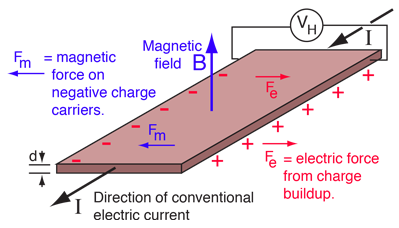
\includegraphics[width=0.5\textwidth]{figures/hall_effect.png}
    \caption{Schematic of a Hall probe measuring the magnetic field. Image gratefully taken from HyperPhysics.\cite{hyperphysics_hall_image}}
    \label{fig:hall_effect}
\end{figure}

The Hall-effect can be used to measure the magnitude of magnetic fields in one direction and is named after Edwin Hall who discovered it in 1879. As \gls{mems}, Hall-effect sensors are a popular alternative to magnetoresistive sensors.\cite{Hall1878}\cite{demtroeder_hall}

The effect is illustrated in Figure \ref{fig:hall_effect}. Magnetic fields exert a transverse force on moving charge carriers. This includes electrical currents in conductors. There, the magnetic field is pushing the charges to one side of the material which is most evident in thin flat conductors. The imbalance of the charges results in a measurable voltage between two sides of the conductor. Its output voltage $V_H$ is directly proportional to the magnetic field strength passing through the sensor, and is equal to:\cite{demtroeder_hall}

\begin{equation}
\label{eq:hall_effect}
    V_H = \frac{I B}{n e d}
\end{equation}

Where $I$ is the current flowing through the probe, $B$ is the magnetic field perpendicular to the probe, $n$ is the charge carrier density, $e$ the elementary charge, and $d$ is the probe thickness.

\section{Earth's magnetic field}
% TODO mention WWM2015 and their 12 harmonic approximation?

The Earth is sourcing a magnetic field from its interior which is reaching out into space, where it interacts with charged particles emitted by the Sun. The magnetic field is believed to be generated by electric currents in conductive convection streams of molten iron and nickel due to heat escaping the Earth's core. This process is complex and an active field of research. On the surface of the Earth, the magnitude of the magnetic flux density ranges from $25$ to $65$ $\mu$T. The field can be approximated by a magnetic dipole tilted at an angle of about $11$ degrees with respect to Earth's rotational axis.\cite{earth_magnetic_bible}\cite{earth_magnetic}

At any location, the Earth's magnetic field can be represented by a three dimensional vector. This is illustrated in Figure \ref{fig:earth_magnetic_field_coords}. A typical procedure for measuring its direction is to use a compass to determine the direction of magnetic North. Its angle relative to true North is called declination or variation. Facing magnetic North, the angle the magnetic field encloses with the horizontal plane is called inclination or magnetic dip. The intensity of the field is proportional to the force it exerts on a magnet. A common representation is X (North), Y (East) and Z (Down) coordinates.\cite{earth_magnetic}\cite{WWM2015}

\begin{figure}[hbt!]
    \centering
    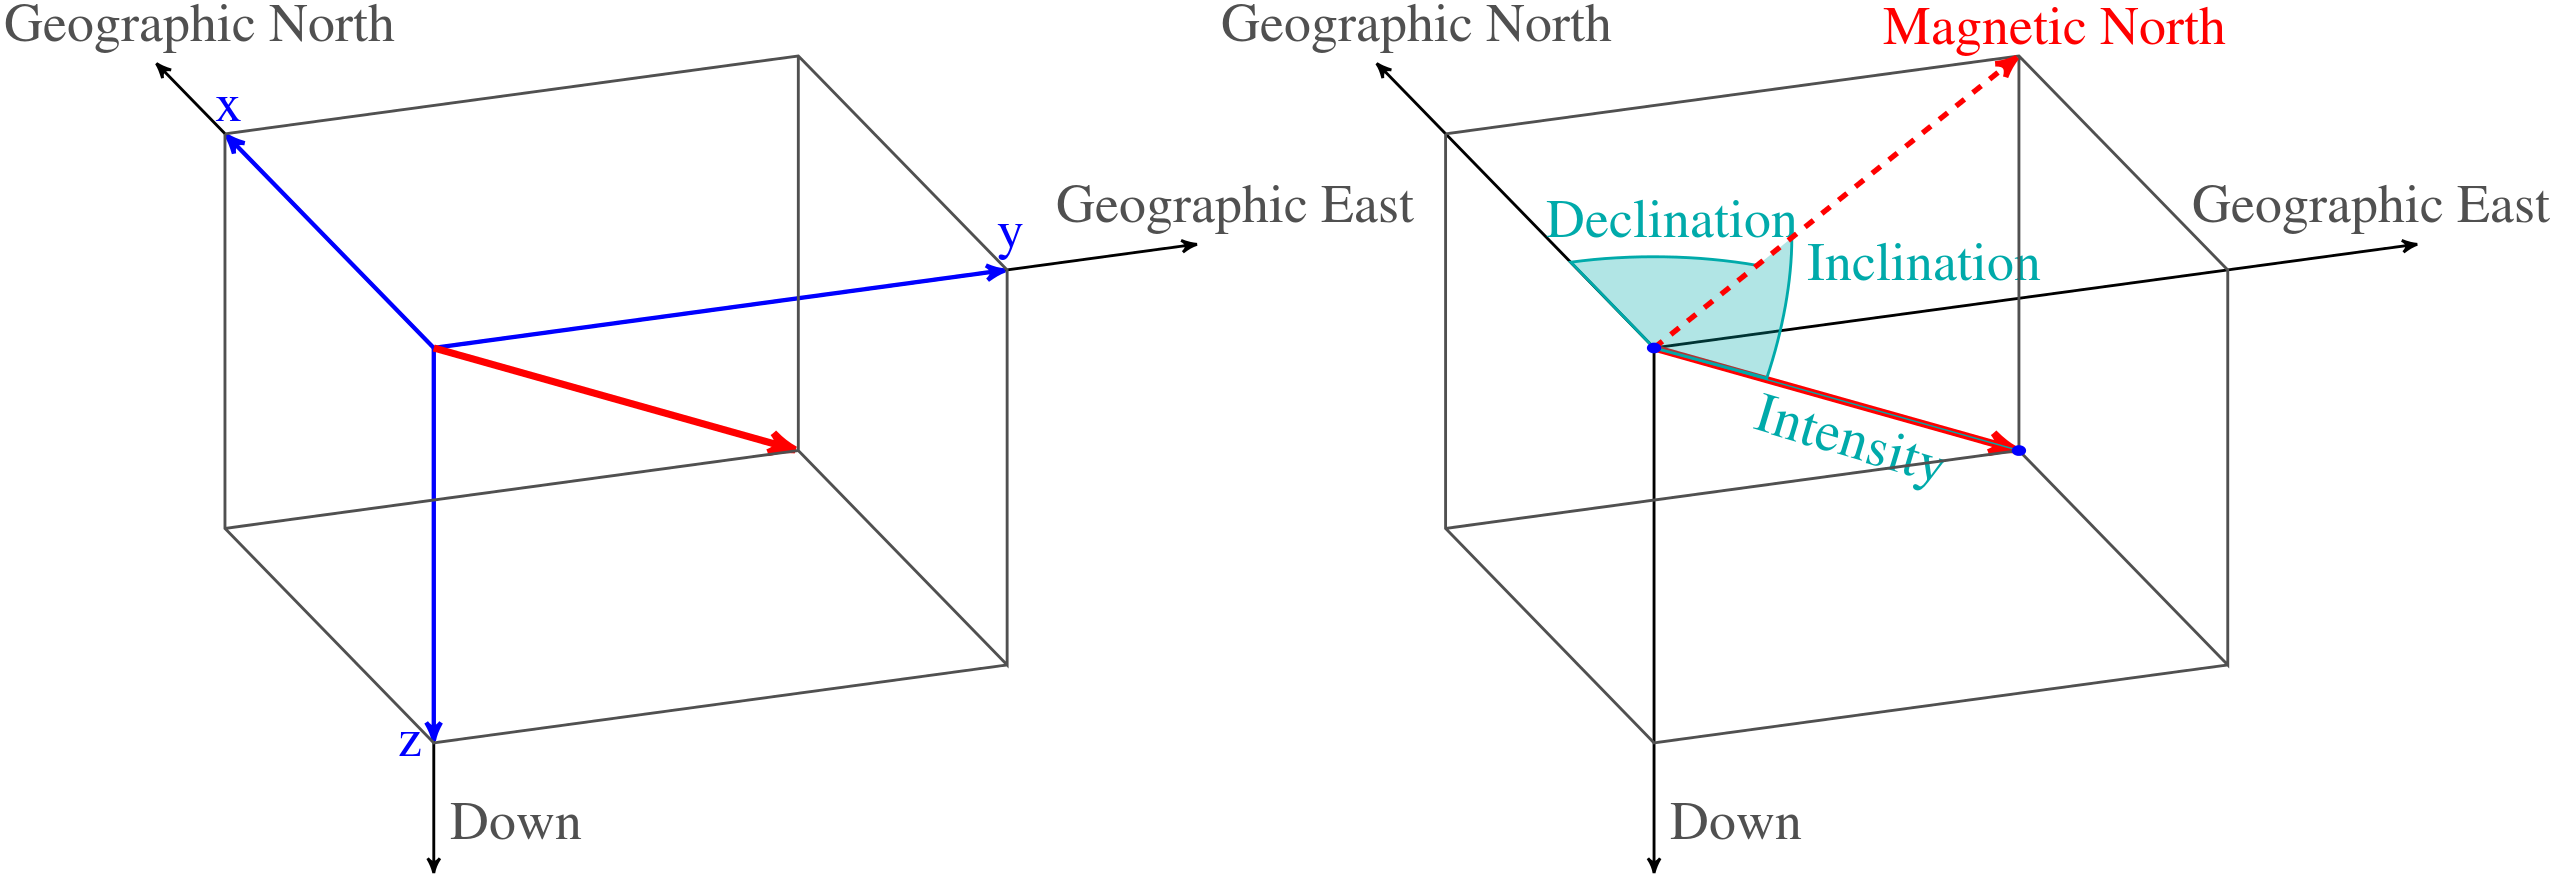
\includegraphics[width=1.0\textwidth]{figures/earth_magnetic_field_coords.png}
    \caption{Common coordinate systems used for representing the Earth's magnetic field. Image gracefully taken from Wikimedia.\cite{wikimedia_magcoords_image}}
    \label{fig:earth_magnetic_field_coords}
\end{figure}

\subsection{Dipole approximation}
\label{subsec:diple_approx}

In close proximity to the surface of the Earth, its magnetic field can be approximated by the field of a magnetic dipole placed at the center of the Earth and oriented with an angle of about $11$ degrees to the rotational axis of the Earth. In this description the Earth can be viewed as a strong bar magnet with its south pole pointing towards the geomagnetic North Pole. The dipole field accounts for approximately 80--90\% of the field in most locations.\cite{earth_magnetic}

In spherical coordinates, the dipole magnetic field of the Earth can be described as follows.\cite{earth_dipole}

\begin{equation}
\label{eq:dipole_approx}
    \begin{aligned}[c]
        B_r &= -2 B_0 ({\frac{R_E}{r}})^3 \cos \theta\\
        B_\theta &= - B_0 ({\frac{R_E}{r}})^3 \sin \theta\\
    \end{aligned}
\end{equation}

Where $B_0$ (typically $B_0 = 3.12*10^{-5}$ T) is the mean value of the magnetic flux density at the magnetic equator on the Earth's surface. $R_E$ is the mean radius of the Earth (approximately $6370\ \textrm{km}$), $r$ is the radial distance from the center of the Earth, and $\theta$ is the azimuth angle measured from the north geomagnetic pole.

This approximation is very practical for our purposes since it is easy to calculate the magnetic flux density for a given WGS84 position.

\section{Quaternions}
% TODO pauli matrices are a possible basis for quaternions
% TODO relation between pauli matrices, SU(2), SO(3)

Quaternions are a number system that extends the complex numbers with two additional imaginary axis. In 1843, they were described by the Irish mathematician William Rowan Hamilton and applied to mechanics in three-dimensional space.\cite{quaternions}

Quaternions are generally represented in the form

\begin{equation}
\label{eq:quaternion}
    \bm{q} = a + b \bm{i} + c \bm{j} + d \bm{k}
\end{equation}

where $a$, $b$, $c$, and $d$ are real numbers, and $\bm{i}$, $\bm{j}$, and $\bm{k}$ are the fundamental quaternion units, similar to the imaginary unit $\bm{i}$.

The imaginary units are connected through multiplication by

\begin{equation}
\label{eq:quaternion_units}
    \bm{i}^2 = \bm{j}^2 = \bm{k}^2 = \bm{ijk} = -1 \textrm{.}
\end{equation}

Quaternions are used in theoretical mathematics and applied mathematics. Applications are calculations involving three-dimensional rotations such as in computer graphics, computer vision, and crystallographic texture analysis. In practical applications, they can be used alongside other methods, such as Euler angles and rotation matrices, or as an alternative to them.

The unit quaternions can be thought of as a choice of a group structure on the 3-sphere $\text{S}^3$ that gives the group $\text{Spin}(3)$, which is isomorphic to $\text{SU}(2)$ and also to the universal cover of $\text{SO}(3)$.

The conjugate of $q$ is given by $q^* = a - b \bm{i} - c \bm{j} - d \bm{k}$.

The norm by $\lVert q\rVert = \sqrt{qq^*} = \sqrt{q^{*}q} = \sqrt{a^2 + b^2 + c^2 + d^2}$.

The inverse by $q^{-1} = \frac{q^*}{\lVert q\rVert ^2}$.

\subsection{Quaternions as rotations}
% TODO mention that a quaternion can be constructed from euler axis+angle?
% TODO mention that all rotations in 3D can be parameterized as euler axis+angle and therefore as quaternion?

To express a rotation of an angle $\theta$ counterclockwise around a unit vector $\bm{u} = u_x \bm{i} + u_y \bm{j} + u_z \bm{k}$ we compose a unit quaternion with the extended Euler's formula

\begin{equation}
\label{eq:euler_ext}
    \bm{q} = e^{{\frac{\theta}{2}}{\bm{u}}} = \cos{\frac{\theta}{2}} + \sin{\frac{\theta}{2} \bm{u}} \textrm{ .}
\end{equation}

In order to apply this rotation to a point $\bm{p} = p_x \bm{i} + p_y \bm{j} + p_z \bm{k}$ one has to compute

\begin{equation}
\label{eq:quaternion_rotation}
    \bm{p}' = \bm{q} \bm{p} \bm{q}^{-1} \textrm{ .}
\end{equation}

Such a rotation is illustrated in Figure \ref{fig:quaternion_rot}.

Rotations can be composed by multiplying quaternions and reversed with the inverse quaternion $\bm{q}^{-1}$.

\begin{figure}[hbt!]
    \centering
    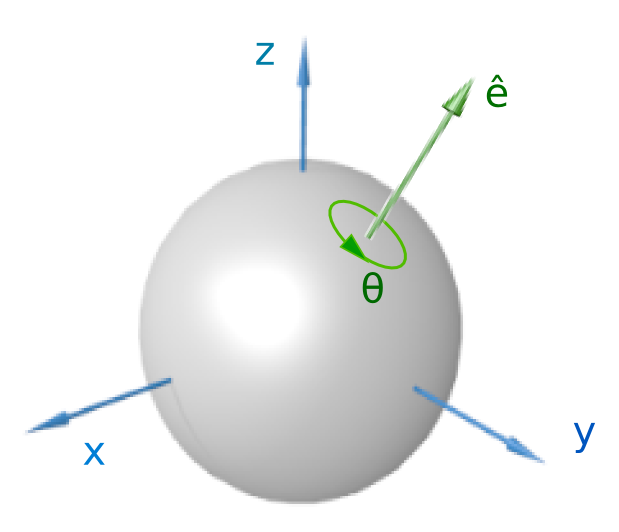
\includegraphics[width=0.5\textwidth]{figures/quaternion_rot.png}
    \caption{Illustration of a rotation represented by an Euler axis and angle. Image gracefully taken from Wikimedia.\cite{wikimedia_euleraxisangle_image}}
    \label{fig:quaternion_rot}
\end{figure}

\section{Bayesian statistics}
\label{sec:bayes}

Bayesian statistics is a theory based on the Bayesian interpretation of probability where it expresses a degree of belief in an event. The degree of belief can be based on prior knowledge about the event, like results of previous experiments, or on personal beliefs about the event. This differs from the frequentist interpretation which views probability as the limit of the relative frequency of an event after many trials.\cite{bayes_1}

Bayes' theorem is used in Bayesian methods to update probabilities after obtaining new data. Given two events $A$ and $B$, the conditional probability $P(A|B)$ -- the probability for $A$ given that $B$ is true -- is expressed as follows:\cite{bayes_1}

\begin{equation}
\label{eq:bayes}
    P(A|B) = \frac{P(B|A)\ P(A)}{P(B)} \textrm{  with  } P(B) \ne 0
\end{equation}

Bayes' theorem is a fundamental result of probability theory, but it has a specific interpretation in Bayesian statistics. In Equation \ref{eq:bayes}, $A$ represents a proposition (prior information like ``this coin lands on heads fifty percent of the time'') and $B$ represents new data we want to take into account (e.g. the result of a series of coin flips). $P(A)$ is the prior probability of $A$, which expresses our beliefs about $A$ before evidence is taken into account. $P(B|A)$ is the likelihood function, which can be interpreted as the probability of the evidence $B$ given that $A$ is true. The likelihood represents the model of the stochastic process and quantifies the extent to which evidence $B$ supports the proposition $A$. $P(A|B)$ is the posterior probability -- the probability of $A$ after taking the evidence $B$ into account. Essentially, Bayes' theorem updates our prior beliefs $P(A)$ after considering new evidence $B$.\cite{bayes_1}

In contrast to the frequentist interpretation, which views probability as the limit of the relative frequency of an event after many trials, Bayesian statistics does not rely on repeatable experiments. There is no true universal value of probability that we want to approach with many trials. Probability is a degree of belief based on data, a model and prior beliefs.


\chapter{Hard Iron Effect}
\label{ch:problem}
% possible refs
%  - https://www.spiedigitallibrary.org/conference-proceedings-of-spie/10445/104455S/Compensation-of-hard--and-soft-iron-distortions-is-magnetometer/10.1117/12.2280794.short
%  - https://www.mathworks.com/help/nav/ref/magcal.html

% this chapter could be split into
%  - (overview)
%  - problem description
%  - related work

% mention that this thesis is about magnetostatics? since building, earth and phone field is changing very slowly (and em waves are far too weak?)

% compare particle filter approach to existing methods
%  - there are some reference about methods in the madgwick internal report

The hard iron effect in the smartphone is caused by magnetic materials inside the phone which retain their magnetism even after the removal of the external magnetic fields. A permanent magnet of a speaker inside the phone, or inside the vibration unit are examples for that. Since the magnetization of the materials can still change in strength and direction in presents of external fields, this is a dynamical effect and therefore needs continuous calibration.

\begin{figure}[hbt!]
    \centering
    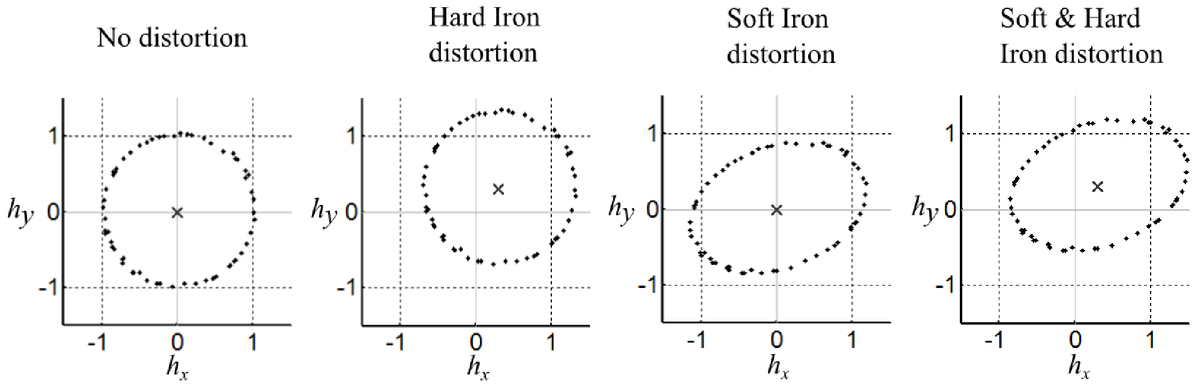
\includegraphics[width=0.6\textwidth]{figures/hard_soft_iron.jpg}
    \caption{Illustration of the hard and soft iron effect.\cite{hard_soft_iron}}
    \label{fig:hard_soft_iron}
\end{figure}

Figure \ref{fig:hard_soft_iron} is an example of how hard and soft iron effects influence the measurement of the magnetometer after a full rotation along an arbitrary axis.

Usually, the hard iron calibration done by the operating system or manufacturer and therefore depending on different algorithms across different devices. Treating the estimates equally is an additional source of error. Apart from that, the operating system does not quantify the quality of the hard iron calibration and requires unnatural movements of the phone to progress the calibration.

The measurement of the magnetic flux density vector by the magnetometer can be expressed by the following.

\begin{equation}
\label{eq:decomposition}
    \bm{B}_{measure} = \bm{B} + \bm{B}_{noise} = \bm{B}_{phone} + \bm{B}_{earth} + \bm{B}_{env} + \bm{B}_{noise}
\end{equation}

Where $\bm{B}_{measure}$ is the measurement of the magnetometer at a given point in time, $\bm{B}_{noise}$ the noise produced by the magnetometer, $\bm{B}_{phone}$ the magnetic field created by the device, $\bm{B}_{earth}$ the magnetic field of the earth, and $\bm{B}_{env}$ is the true ambient magnetic field of the environment.

Let us imagine to rotate the phone in any direction to understand how the individual components change. Assuming that $\bm{B}_{noise}$ is isotropic it will not change. In the frame of reference of the phone, $\bm{B}_{earth}$ and $\bm{B}_{env}$ will be rotated in the opposite direction. The magnetic field of the device $\bm{B}_{phone}$ is created by components of the interior which are firmly connected to the magnetometer. Therefore $\bm{B}_{phone}$ is constant in the frame of reference of the device.

Since $\bm{B}_{earth}$ and $\bm{B}_{env}$ behave in the same way under rotation of the device, we can already guess that the full decomposition is a non trivial problem. Assuming we know the horizontal and vertical component of $\bm{B}_{earth}$ (those could be calculated with the dipole approximation of the Earth's magnetic field) it only depends on the horizontal orientation of the device. Without any model for $\bm{B}_{env}$ the decomposition is ambiguous in all directions. Such a model would make assumptions about the magnitude (for example $\lVert \bm{B}_{env} \rVert << \lVert \bm{B}_{earth} \rVert$) or direction (for example random directions) for the ambient magnetic field of the environment.

Common calibration techniques are:

\begin{itemize}
  \item Static calibration. The device is rotated in all directions while measuring the magnetic field and orientation of the device. A numerical fit can be used to estimate the hard iron effect and these values will later be used in the application to correct the measurements.
  \item Calibration by significant rotation. An algorithm detects when the phone is rotated significantly in multiple directions and uses the same approach as above to estimate the hard iron effect.
\end{itemize}


\chapter{Particle Filter}
\label{ch:particle}
% TODO maybe use figures and examples across the chapter

This chapter is a short introduction to \gls{smc} methods and specifically particle filters. First, we give an overview about particle filters and state-space models. Then we will derive the recursive filtering equations by following Bayes' theorem. At the end, we will introduce resampling and point out why it is a crucial feature of \gls{smc} methods.

\section{Overview}

The term \textit{filtering} in this context means extracting information about a signal from partial and noisy observations in dynamical systems. In contrast to other estimation problems, filtering is about estimating the current state of a system given only observations up to this point in time.\cite{AppliedOptimalEstimation}

Particle filters were originally developed for object tracking and time series analysis for nonlinear, non-Gaussian state-space models.\cite{Gordon1993} The term particle filter was first used by Del Moral in 1996.\cite{Moral1996}

Particle filters are \gls{smc} methods and a subset of \gls{mc} algorithms. They can be used to solve filtering problems arising in signal processing and Bayesian statistical inference. The goal is to compute the posterior distributions of states in a Markov process, given the prior distribution of states and some partial and noisy observations.

The particle filter uses a set of particles to represent the current state of the system. There is no limitation to the state-space model, the initial state, and the noise distribution of observations. However, in practice the particle filter does not perform well in very high-dimensional systems.

Each particle has a weight (or likelihood) that represents an approximate probability measure of that particle being sampled from the usually analytically unknown probability density function. The weights are updated when new evidence about the true state is available. A resampling step is necessary to avoid weight disparity leading to weight collapse. There are several adaptive resampling criteria that can be used to reduce noise, including the variance of the weights and the relative entropy with respect to the uniform distribution. In the resampling step, the particles with negligible weights are replaced by new particles in the proximity of the particles with higher weights.\cite{Moral1996}\cite{Moral2012}

\section{Filtering with state-space models}

According to Hans Künsch\cite{Kuensch2013}, in the last 50 years filtering has been mainly studied in the framework of state-space or hidden Markov models, assuming a Markovian time evolution of the signal and observations, which are instantaneous functions of the signal, and subject to white observation noise.

The objective of a filter is to estimate the hidden state variables $X_k$ (also called signal) given the observation variables $Y_k$ at iteration $k$. The observable variables $Y_k$ are related to the hidden variables $X_k$ by some conditional probability density $g(y_k|x_k)$ that is known. Similarly, the dynamics of the state process is also known $f(x_k|x_{k-1})$. A generic state and observation process is illustrated below.

\[\begin{array}{cccccccccc}
X_0 & \to & X_1 & \to & X_2 & \to & X_3 & \to & \cdots & \text{signal} \\
\downarrow & & \downarrow & & \downarrow & & \downarrow & & \cdots & \\
Y_0 & & Y_1 & & Y_2 & & Y_3 & & \cdots & \text{observation}
\end{array}\]

Given the sequential observations $Y_0,\cdots,Y_k$ at any time step $k$, the filtering problem is to estimate the signal $X_k$.

Bayesian estimates of $X_k$ follow from the posterior density $p(x_k|y_0,\cdots,y_k)$. Particle filters provide an approximation of these conditional probabilities by weighted samples. In contrast to \gls{smc} methods, \gls{mcmc} methods would have to deal with the full posterior distribution $p(x_0,\cdots,x_k|y_0,\cdots,y_k)$ in each iteration.

\section{Filtering recursion}

In order to start the recursion, a prior distribution $p(x_0)$ of the signal $X_0$ is required. Selecting samples of the prior distribution is called initialization. One has to be careful choosing a prior distribution because it might cause bias. The prior could depend on the first observation $Y_0$ for example.

At time step $k=1$ we observe $Y_1$ and want to update the filter. Following Bayes' theorem (see Equation \ref{eq:bayes} in Section \ref{sec:bayes}) we derive the following:

\begin{equation}
\label{eq:pf_1}
    p(x_0,x_1|y_1) \sim L(y_1|x_0,x_1)\ p(x_1) = g(y_1|x_1)\ f(x_1|x_0)\ p(x_0)
\end{equation}

Where $L(y_1|x_0,x_1)$ is the likelihood function given by the observation function $g(y_k|x_k)$ and $p(x_1)$ is the prior for $X_1$ given by the signal prediction function $f(x_k|x_{k-1})$ and $p(x_0)$. Following this process recursively and applying normalization yields the following:

\begin{equation}
\label{eq:pf}
    p(x_{1:k}|y_{1:k}) = \frac{g(y_k|x_k)\ f(x_k|x_{k-1})\ p(x_{1:k-1}|y_{1:k-1})}{p(y_k|y_{1:k-1})}
\end{equation}

\begin{equation}
\label{eq:pf_norm}
    p(y_k|y_{1:k-1}) = \int_{S} g(y_k|x_k)\ f(x_k|x_{k-1})\ p(x_{1:k-1}|y_{1:k-1}) \,dx_k
\end{equation}

With the abbreviation $x_{1:k} = x_1,\cdots,x_k$, the normalization $p(y_k|y_{1:k-1})$ in Equation \ref{eq:pf_norm}, and the state space volume $S$.

By marginalization of \ref{eq:pf} (integration over $x_{1:k-1}$) we derive the following:

\begin{equation}
\label{eq:pf_update}
    p(x_k|y_{1:k}) = \frac{g(y_k|x_k)\ p(x_k|y_{1:k-1})}{p(y_k|y_{1:k-1})}\
\end{equation}

\begin{equation}
\label{eq:pf_prediction}
    p(x_k|y_{1:k-1}) = \int_{V} f(x_k|x_{k-1})\ p(x_{k-1}|y_{1:k-1}) \,dx_{k-1}
\end{equation}

Equation \ref{eq:pf_prediction} is usually called the prediction step and \ref{eq:pf_update} the update step. However, according to Arnaud Doucet\cite{Doucet2011} most particle filtering methods rely on numerical approximations of \ref{eq:pf} instead of \ref{eq:pf_prediction} and \ref{eq:pf_update}.

Analytical solutions can be given for two important special cases. First, when the state space $S$ is finite, the integrals above can be reduced to finite sums. Second, when the system is linear and $p(x_0)$, $g(y_k|x_k)$, and $f(x_k|x_{k-1})$ are Gaussian, the filtering problem can be solved by a Kalman filter exactly.\cite{Kalman1960}

\section{Resampling}
\label{sec:pf_resampling}

An algorithm that follows the initialization, prediction, and update steps sequentially by representing the distributions with $N$ samples is called \gls{sis}. It can be shown that the variance of the weights is growing exponentially with the number of iterations. The important and defining feature of particle filters is the resampling step, which removes particles with low weights and replaces particles with high weights by multiple offspring particles in close proximity. After a resampling step, all particles have the same weight and the distribution is only represented by the number of particles in the different states.\cite{Doucet2011}

Common algorithms for resampling are \textbf{systematic resampling} and \textbf{multinomial resampling}. Both require a summation of all weights which can be a bottleneck for parallelization. Other techniques were discussed by Murray, Lee, and Jacob in 2016.\cite{Doucet2011}\cite{parallel_resampling}

Adaptive resampling can be used to reduce noise and avoid unnecessary resampling steps in case of a sufficiently even weight distribution. A popular criteria is the effective number of particles.

\begin{equation}
\label{eq:pf_effective}
    {\hat{N}}_{\mathit{eff}} = \frac{1}{\sum_{i=1}^N\left(w_i\right)^2} \leq N_\mathit{thr}
\end{equation}

With normalized weights \(\sum_{i=1}^N{w_i} = 1\) and the threshold parameter $N_\mathit{thr}$.\cite{Moral2012}


\chapter{Implementation}
\label{ch:impl}
This chapter walks through the chosen technologies, shows the architecture, frames the implementation effort, and explains the decisions taken while working on this thesis. First we will introduce the different technologies and how they play together. Second we will shortly define the frames of reference and the architecture of the implementation. Then the particle filter implementation will be explained in detail, followed by the filter routine and its parameters. Afterwards a few intermediate steps and solved issues that should come up while working on this thesis are discussed. Finally the platform implementation in case of Android and the effort made on visualization is described.

In order to design, implement and evaluate an online hard iron calibration, two different approaches were taken into consideration. Approach \textit{One}: using existing tools to collect the required sensor data and to process and evaluate it offline. Approach \textit{Two}: designing a system from scratch that collects, processes and visualizes sensor data in real time. Since the outcome of this thesis should be an online algorithm and it seemed to be more target-oriented, the prototyping was created with the paradigm of approach \textit{Two}. Moreover, the orientation estimation (see Section \ref{sec:ori_est}) required qualitative evaluation which was preferable in the online scenario because of the immediate response in the visualization. Approach \textit{One} was later used for the quantitative evaluation of the hard iron calibration.

\section{Technology}

The major criteria for the choice of technology was \textit{platform independence} and \textit{real-time processing}. Platform independence because we are targeting two different mobile platforms with Android and iOS and the need of an evaluation framework that runs on a desktop environment like Ubuntu. Since our calibration should be online, real-time processing is necessary and therefore a critical performance limit is attached to our problem: When one second of real-time has passed we have to process at least one second of input data.

Visualization was planned for prototyping and evaluation purposes. Similar to our calibration algorithm, the visualization was planned to be platform independent with the benefit of displaying it on the smartphone and on the desktop by the same implementation. The first attempt was to use OpenGL from C++ but that introduced a lot of overhead to the implementation. Since all target platforms have an HTML5 compatible browser, the second and final attempt was to use JavaScript for that purpose. To communicate with C++ in real-time, WebSocket was used to exchange Protocol Buffers (see Subsection \ref{sec:protobuf}).

The target platform for the demo application was chosen to be Android. It was developed in Java, responsible for reading the sensors and providing a small user interface.

Table \ref{tbl:code_lines} gives a quick overview about the chosen technologies and the implementation effort by lines of code.

\begin{table}[h]
    \centering
    \begin{tabular}{ | l | r | }
    \hline
    \textbf{Language} & \textbf{Total lines of code} \\ \hline
    C++               & 3092 \\ \hline
    Java              &  366 \\ \hline
    JavaScript        &  450 \\ \hline
    Python            &  179 \\ \hline
    Protocol Buffers  &   55 \\ \hline
    CMake             &  203 \\ \hline
    \end{tabular}
    \caption{Total lines of code by language written for this thesis.}
    \label{tbl:code_lines}
\end{table}

\subsection{C++}

The programming language that was used the most in this project is C++ for various reasons. C++ is platform independent and can reach major smartphone platforms like Android and iOS. Performance was critical for the implementation which is a major purpose of C++. Since C++11 there is a sufficient standard library for common data structures, random variables and common algorithms. Besides that, C++ is a modern programming language with multiple paradigms for example it is object-oriented and generic.

Along with C++ multiple tools, frameworks, and libraries were used which are shortly described in the following.

\begin{itemize}
  \item \textbf{boost} is a popular C++ library that comes in handy where the standard library is missing functionality. This thesis only depends on \textbf{boost asio} for networking and \textbf{boost beast} for HTTP and WebSocket.
  \item \textbf{Eigen} is a rich library for linear algebra and comes with implementations for matrices, vector, and quaternions.
  \item \textbf{gtest} is a unit test framework from Google and was used to write small self-contained (unit) test cases.
  \item \textbf{CMake} was used as dependency management and build system.
\end{itemize}

\subsection{Android}

Android is a mobile operating system based on a modified version of the Linux kernel and other open source software. It was primarily designed for mobile devices with touchscreen such as smartphones and tablets. Android is developed by a consortium of developers known as the Open Handset Alliance and commercially sponsored by Google. It was unveiled in November 2007, with the first commercial Android device launched in September 2008.

Android has been the best-selling \gls{os} worldwide on smartphones since 2011 and on tablets since 2013. As of May 2017, it has over two billion monthly active users, which is the largest installation base of any operating system.

Android is one of the target platforms for this thesis. Native applications can be developed with Android Studio in Java or Kotlin. Moreover, C++ can be integrated and called through \gls{jni} for shared library access, enabling low-level functionality and high performance applications.

\subsection{JavaScript}

JavaScript was used to realize platform independent visualization that can be displayed on desktop and mobile devices. In contrast to the original approach via OpenGL it was more straight forward to use with \textbf{plotly}\footnote{High level plotting library for Javascript and Python. \url{https://plotly.com/}} and a \textbf{matplotlib}\footnote{High level plotting library for Python. \url{https://matplotlib.org/}} background in Python. Moreover, modern browsers come with a WebSocket implementation which reduced the complexity of communication to C++ code.

Along with JavaScript multiple tools, frameworks, and libraries were used which are shortly described in the following.

\begin{itemize}
  \item \textbf{webpack} is a module bundler. Its main purpose is to bundle JavaScript files for usage in a browser.
  \item \textbf{plotly} is a rich plotting library for JavaScript and Python and was used for visualization purposes.
  \item \textbf{THREE} is a library for linear algebra and comes with implementations for matrices, vector, and quaternions.
\end{itemize}

\subsection{Protocol Buffers}
\label{sec:protobuf}

Protocol Buffers\footnote{\url{https://developers.google.com/protocol-buffers}} (short Protobuf) are Google's language-neutral, platform-neutral, extensible mechanism for serializing structured data. It is useful for programs which communicate over a wire or for storing data. Protocol Buffers involve an interface description language which defines the structure of the data. Additionally it comes with a program that generates source code from that definition. The generated code deals with the encoding and decoding of byte streams which represent the structured data.

The data can be serialized in binary representation which takes up less space compared to a text representation like JSON. Therefore it needs less bandwidth while communicating over network.

\section{Frame of reference}
% quaternion transforms from what to what?
% TODO ref images https://developer.android.com/reference/android/hardware/SensorEvent

An important choice while dealing with sensors that have spatial orientation is the frame of reference. Two frames had to be chosen. A local one for the phone and its sensors and a global one for the user and his environment. The chosen axis for the frames of reference are shown in Figure \ref{fig:frames_of_reference} and align with those defined in the Android sensor SDK. While magnetometer readings are taken in the phone's frame of reference it is important to transform those measurements to the global frame of reference since there the magnetic field is expected to be constant in close proximity.\cite{android_sdk_sensorevent}

The transformation between those two frames is estimated by the orientation filter which forms an \gls{imu} based on the accelerometer and gyroscope. While the accelerometer provides information about two orientation angles, the gyroscope can be used to make the estimate more reliable. Additionally, with the gyroscope we can give an relative estimate about the horizontal orientation between two points in time. That angle will drift due to measurement errors which accumulate over time essentially generating a random walk.

In this thesis an algorithm designed by Madgwick was used to estimate the orientation of the phone. See Section \ref{sec:ori_est} for further details.

\begin{figure}[hbt!]
    \centering
    \begin{subfigure}{0.4\textwidth}
        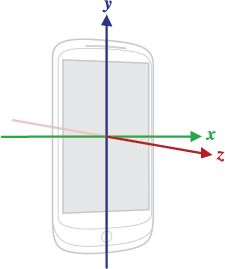
\includegraphics[height=1.0\linewidth]{figures/coords_phone.png}
        \caption{}
    \end{subfigure}
    \begin{subfigure}{0.4\textwidth}
        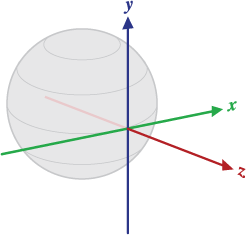
\includegraphics[height=1.0\linewidth]{figures/coords_global.png}
        \caption{}
    \end{subfigure}
    \caption{Chosen frames of reference. With (a) the \textit{local frame of reference} or \textit{device coordinates} and (b) the \textit{global frame of reference} or \textit{world coordinates}. Gracefully taken from Android documentation.\cite{android_sdk_sensorevent}}
    \label{fig:frames_of_reference}
\end{figure}

\section{Software architecture}

Since the implementation was growing fast in complexity, it was important to structure the project into logical and modular components. A lot of thoughts went into code architecture and design decisions which will be shortly discussed here.

The desired architecture had to deal with multiple programming languages and potential concurrency issues. Moreover, algorithms should be modules that only depend on their input and output which makes it easy to swap them and to test them in a generalized way. Another advantage could be the ability to systematically detect bottle necks.

The different algorithms ended up as plugable components in a pipelining scheme. Sensor and filtered data is passed through pipes from processing entity to processing entity. These processing entities were called nodes. The architecture was applied to the C++ code and the messaging protocol defined with Protocol Buffers. It was also applied in JavaScript but in a more simplified fashion. On Android, Java was used to call \gls{jni} wrapper functions to C++ and therefore did not require any particular architecture.

The overall architecture and different modules are shown in Figure \ref{fig:architecture}.

\begin{figure}[hbt!]
    \centering
    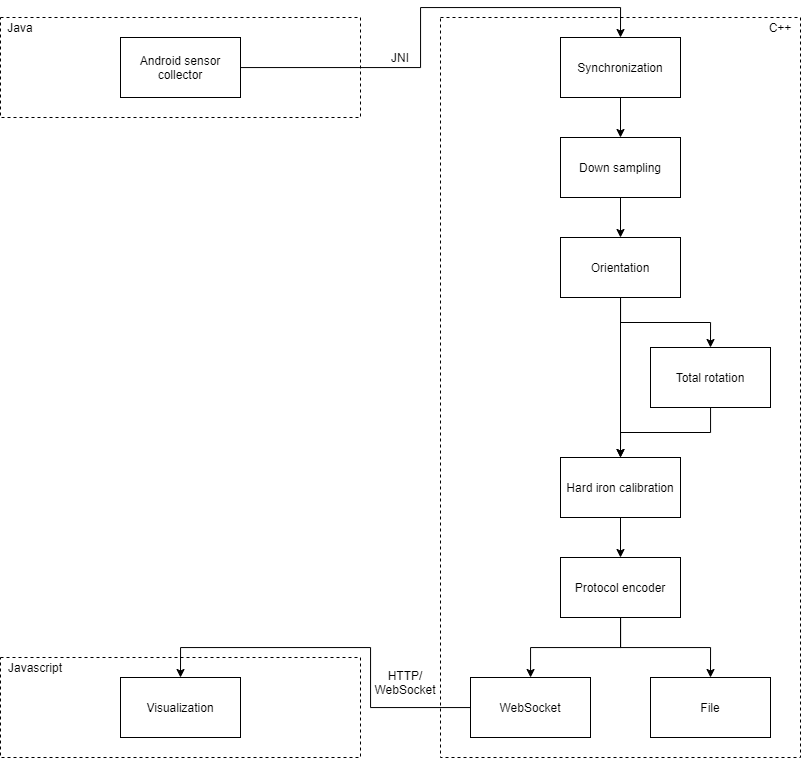
\includegraphics[width=1.0\textwidth]{figures/architecture.png}
    \caption{Illustration of the software architecture grouped by programming language.}
    \label{fig:architecture}
\end{figure}

\section{Particle filter}
\label{sec:impl_pf}
% TODO refer to particle filter section?

In the following subsections we will walk through the different components of the particle filter. First, potential numerical issues with likelihoods are discussed. Second, the representation of a single particle in the filter is presented. Afterwards, the initialization, propagation, update, and resampling steps are discussed. Finally, we will see how the hidden states are estimated.

The bootstrap particle filter\cite{Doucet2011}\cite{Kuensch2013} was chosen as a template for the following implementation.

Initially, the particle filter was designed to model the complete decomposition given in Equation \ref{eq:decomposition} and \ref{eq:decomposition_earth_env}. Since $\bm{B}_\text{earth}$ and $\bm{B}_\text{env}$ transform in the same way under rotation of the device and we do not have a model for $\bm{B}_\text{env}$ this approach failed. The particle filter was further simplified to only decompose Equation \ref{eq:decomposition}.

\subsection{Likelihood}

In Bayesian statistics, likelihood is the key to model the update from a prior to a posterior distribution. Since we do this numerically, we have to be careful with the numerical limitations of the underlying machine. We expect single-precision floating-points as IEEE 754-1985 with the following properties: 1 sign bit, 8 exponent bits, 23 significant precision bits. This leads to an exponent int the range $[-126,127]$. Since likelihood arithmetic involves multiplications with very small numbers we have to use the log likelihood instead.

To calculate the weights from the log likelihood we used the largest log likelihood involved and subtract it from all log likelihoods. This is possible because the weights are invariant under scalar multiplication as a relative measure and can be renormalized if necessary. Additionally this technique maps the weights to numbers in the range $[0,1]$.

\subsection{One particle}

One particle represents the state of one realization of the hard iron calibration. Table \ref{tbl:one_particle} summarizes the properties of one particle. The calibration can be parameterized with a three dimensional vector representing the offset of the measurement from the true value. Another vector keeps the estimated external field, denoted by $\bm{B} = \bm{B}_\text{measure} - \bm{B}_\text{phone}$ with $\bm{B}_\text{phone}$ as the hard iron offset. The external field will later be compared to the next estimate to check for consistency. We also store the \textsc{logLikelihood} later also denoted by $\ell$ and the \textsc{weight} later also denoted by $\mathcal{W}$. They are related to each other but it is handy to keep them separate. Moreover, this might have performance advantages since we do not need to convert between them all the time.

\begin{table}[h]
    \centering
    \begin{tabular}{ | l | p{10cm} | }
    \hline
    \textbf{Field}             & \textbf{Description} \\ \hline
    \textsc{hardIron}          & The hard iron offset represented by this particle. \\ \hline
    \textsc{external}          & The external magnetic field $\bm{B}$ consistent with the last measurement. \\ \hline
    \textsc{logLikelihood}     & Logarithm of the likelihood $\ell$ of this particle. \\ \hline
    \textsc{weight}            & The weight $\mathcal{W}$ of this particle which describes how likely this realization is. It is a relative measure to the total weight among all particles. \\ \hline
    \end{tabular}
    \caption{Description of the properties of one particle.}
    \label{tbl:one_particle}
\end{table}

\subsection{Initialization}

The particle filter has to be initialized with a prior distribution for the hard iron calibration. Pseudocode for the initialization step is given in Algorithm \ref{alg:pf_init}. Without taking further assumptions, a Gaussian distribution $\text{N}(0, \sigma^2)$ was chosen to sample each component of the hard iron vector. In order to enforce the constraint $\bm{B}_\text{measure} = \bm{B}_\text{phone} + \bm{B}$ (see Equation \ref{eq:decomposition}), we need an initial magnetometer observation $\bm{B}_\text{measure}$.

Two potential improvements to the initialization were identified. First, if the device was calibrated in the past, we could choose that as the center of our distribution or mix it with the one at the origin. Second, the current calibration of the operating system might also be a reasonable starting point of our calibration.

\begin{algorithm}[h]
	\KwIn{population size $N$, hard iron variance $\sigma^2$, magnetic field measurement $\bm{B}_\text{measure}$, orientation $\bm{q}$}
	\KwOut{initialized and populated particle filter $P$}
	$P \leftarrow$ \textsc{allocateParticles}($N$)\\
	\ForEach{particle in $P$}{
		$\bm{B}_\text{phone} \leftarrow$ \textsc{gaussianDrawThree}($0$, $\sigma^2$)\\
		\smallskip
		$\bm{B} \leftarrow q \times (\bm{B}_\text{measure} - \bm{B}_\text{phone})$\\
		\smallskip
		$\ell \leftarrow -\log{N}$\\
		\smallskip
		$\mathcal{W} \leftarrow \frac{1}{N}$\\
	}
	\Return{$P$}
	\caption{Initialization of the particle filter as pseudocode.}
	\label{alg:pf_init}
\end{algorithm}

\subsection{Prediction}

In order to predict future states of our particles we have to apply the state transition. Pseudocode for the propagation step can be found in Algorithm \ref{alg:pf_prop}. Since we do not have a physical model for the time evolution of the hard iron effect, the idea was to apply a random walk for each particle. This approach allows the particle filter to do recalibration over time.

\begin{algorithm}[h]
	\KwIn{population $P$, time passed $t$, hard iron variance drift rate $\sigma^2$}
	\KwOut{population $P$}
	\ForEach{particle in $P$}{
		$\bm{B}_\text{phone} \leftarrow \bm{B}_\text{phone}$ + \textsc{gaussianDrawThree}($0$, $t * \sigma^2$)\\
	}
	\Return{$P$}
	\caption{Prediction step of the particle filter as pseudocode.}
	\label{alg:pf_prop}
\end{algorithm}

\subsection{Update}

We update our particle filter by feeding it with new observations from the magnetometer and new estimates of the orientation filter (see Section \ref{sec:ori_est}). Pseudocode for the update step is given in Algorithm \ref{alg:pf_update}. We predict the measurement of the magnetic field $\bm{B}_\text{measure}$ by transforming the previous estimate of the external field $\bm{B}$ into the local frame of reference and adding the hard iron vector $\bm{B}_\text{phone}$. Based on that prediction $\hat{\bm{B}}_\text{measure}$ and the measurement $\bm{B}_\text{measure}$, a likelihood can be calculated. That likelihood was modeled by a Gaussian distribution $N(0, \sigma^2)$. $\sigma^2$ can be used to parameterize the noise of the sensor and the variation of the magnetic field between two different points in space.

\begin{algorithm}[hbt!]
	\KwIn{population $P$, magnetic field measurement $\bm{B}_\text{measure}$, orientation $\bm{q}$, prediction variance $\sigma^2$}
	\KwOut{population $P$}
	\ForEach{particle in $P$}{
	    $\hat{\bm{B}}_\text{measure} \leftarrow \bm{B}_\text{phone} + \bm{q}^{-1} \times \bm{B}$\\
	    $\ell \leftarrow \ell +$ \textsc{gaussianLogPDF}($\hat{\bm{B}}_\text{measure}$, $\bm{B}_\text{measure}$, $\sigma^2$)\\
	    $\bm{B} \leftarrow \bm{q} \times (\bm{B}_\text{measure} - \bm{B}_\text{phone})$\\
	}
	\Return{$P$}
	\caption{Update step of the particle filter as pseudocode.}
	\label{alg:pf_update}
\end{algorithm}

\subsection{Resampling}
% TODO refer to particle filter section?

The resampling step is the most important part of the particle filter. Without it the likelihood would converge to zero and the variance of the weights would only increase. The idea is to remove unlikely states and replace them with more likely ones. The chosen algorithm, called multinomial resampling\cite{Doucet2011}\cite{parallel_resampling}, is a common resampling algorithm with a time complexity of $\mathcal{O}(n \ln{n})$ and memory complexity of $\mathcal{O}(n)$.\cite{particle_resample}

Pseudocode for the resampling step is given in Algorithm \ref{alg:pf_resampling}. First we calculate the weight of each particle $\mathcal{W}$ by its likelihood $\ell$. Then we accumulate these weights into an array of partial sums $w_i$. Now we can draw uniformly distributed samples $x$ from the range $0$ to total weight $\mathcal{W}_{sum}$ and lookup the lower bound elements in the array. Thereby we get the indices $i$ of the particles we are going to sample from. We copy the state of those particles $P_{in}^{i}$ into a second array and afterwards exchange it with the previous array of particles (double buffering).

Since the propagation step applies a random walk to the hard iron offset, we do not have to worry about state degeneracy.

\begin{algorithm}[h]
	\KwIn{population $P_{in}$, population size $n$}
	\KwOut{population $P_{out}$}
	$\ell_{max} \leftarrow \textsc{max}(\ell)$\\
	$\mathcal{W}_{sum} \leftarrow 0$\\
	$w \leftarrow$ \textsc{allocateFloats}($n$)\\
	\ForEach{$p$ in $P_{in}$}{
	    $\mathcal{W} \leftarrow e^{\ell - \ell_{max}}$\\
	    $\mathcal{W}_{sum} \leftarrow \mathcal{W}_{sum} + \mathcal{W}$\\
	    $w_i \leftarrow \mathcal{W}_{sum}$\\
	}
	\ForEach{$p$ in $P_{out}$}{
	    $x \leftarrow$ \textsc{random}($0$, $\mathcal{W}_{sum}$)\\
	    $i \leftarrow$ \textsc{lowerBounds}($w$, $x$)\\
	    $p \leftarrow P_{in}^{i}$\\
	}
	\Return{$P_{out}$}
	\caption{Resampling step of the particle filter as pseudocode.}
	\label{alg:pf_resampling}
\end{algorithm}

\subsection{Estimation}

In the estimation step we want to measure the hidden state of our system. The state of the particle filter is represented by its population, the particles, and their states and weights.

Pseudocode for the estimation step is given in Algorithm \ref{alg:pf_estimate}. In order to get an estimate of the hard iron vector and its error, a weighted average and weighted covariance matrix is calculated from the population of the filter. The covariance matrix can later be used to quantify the convergence of the filter.

\begin{algorithm}[h]
	\KwIn{population $P$}
	\KwOut{hard iron vector $\bm{\hat{B}}_{phone}$, hard iron covariance $\bm{\hat{\Sigma}}_{phone}$, external magnetic field vector $\bm{\hat{B}}$, external magnetic field covariance $\bm{\hat{\Sigma}}$}
    $\bm{\hat{B}}_{phone} \leftarrow$ \textsc{weightedAverage}($P$, $\mathcal{W}$, $\bm{B}_\text{phone}$)\\
    $\bm{\hat{\Sigma}}_{phone} \leftarrow$ \textsc{weightedCovariance}($P$, $\mathcal{W}$, $\bm{B}_\text{phone}$)\\
    $\bm{\hat{B}} \leftarrow$ \textsc{weightedAverage}($P$, $\mathcal{W}$, $\bm{B}$)\\
    $\bm{\hat{\Sigma}} \leftarrow$ \textsc{weightedCovariance}($P$, $\mathcal{W}$, $\bm{B}$)\\
	\Return{$\bm{\hat{B}}_\text{phone}$, $\bm{\hat{\Sigma}}_\text{phone}$, $\bm{\hat{B}}$, $\bm{\hat{\Sigma}}$}
	\caption{Estimation step of the particle filter as pseudocode.}
	\label{alg:pf_estimate}
\end{algorithm}

\section{Filter routine}

Our filter routine for the hard iron calibration is a combination of all the steps described in Section \ref{sec:impl_pf}. The parameters of the filter are summarized in Table \ref{tbl:impl_params}.

\begin{table}[h]
    \centering
    \begin{tabular}{ | l | p{10cm} | }
    \hline
    \textbf{Parameter}       & \textbf{Description} \\ \hline
    \textsc{seed}                   & Seed for the pseudorandom number generator. \\ \hline
    \textsc{population}             & The total number of particles. \\ \hline
    \textsc{deltaTime}              & The time difference in seconds between two filter iterations. \\ \hline
    \textsc{initialVariance}        & The initial hard iron variance for the initialization procedure in $(\mu T)^2$. \\ \hline
    \textsc{driftRate}              & The hard iron calibration drift rate for the propagation procedure. \\ \hline
    \textsc{predictionVariance}     & The prediction variance for the update procedure in $(\mu T)^2$. \\ \hline
    \textsc{minimalRotation}        & Minimal rotation angle to perform an update in radians. \\ \hline
    \textsc{resamplingRate}         & Relative amount of effective particles to trigger resampling. \\ \hline
    \end{tabular}
    \caption{Parameter description of the filter.}
    \label{tbl:impl_params}
\end{table}

Pseudocode of the filter routine is given in Algorithm \ref{alg:routine}. We initialize the filter with the first observations of the magnetometer and orientation filter. Then we update and propagate based on time passed and newly incoming observations. The filter will only update after significant rotations which is parameterized by \textsc{minimalRotation}. This has the benefit of saving \gls{cpu} consumption and filtering noise of the orientation estimation which could result in biased hard iron estimates. Adaptive resampling (see Equation \ref{eq:pf_effective} in Section \ref{sec:pf_resampling}) is used to reduce noise, might spare \gls{cpu} usage and can be parameterized with \textsc{resamplingRate}.

\begin{algorithm}[h]
	\KwIn{magnetic field measurement $\bm{B}_\text{measure}$, orientation $\bm{q}$}
	\KwOut{calibrated magnetic field $\bm{\hat{B}}$, calibrated magnetic field covariance $\bm{\hat{\Sigma}}$}
	\If{\textsc{notInitialized()}}{
	    $P \leftarrow$ \textsc{init}($\bm{B}_\text{measure}$, $\bm{q}$)\\
	    \textsc{estimate}()\\
	}
	\If{\textsc{significantRotation()}}{
	    \textsc{update}($\bm{B}_\text{measure}$, $\bm{q}$)\\
	    $\bm{\hat{B}}_{phone}$, $\bm{\hat{\Sigma}}_{phone}$ $\leftarrow$ \textsc{estimate}()\\
	    \If{\textsc{effectiveParticles()} < \textsc{population} $\times$ \textsc{resamplingRate}}{
	        \textsc{resample}()\\
	    }
	}
	$\bm{\hat{B}} \leftarrow \bm{B}_\text{measure} - \bm{\hat{B}}_{phone}$\\
    $\bm{\hat{\Sigma}} \leftarrow \bm{\hat{\Sigma}}_{phone}$\\
	\Return{$\bm{\hat{B}}$, $\bm{\hat{\Sigma}}$}
	\caption{The filter routine as pseudocode.}
	\label{alg:routine}
\end{algorithm}

\section{Synchronization}
\label{sec:impl_synchro}

Our work targets mobile devices with Android and iOS. Since those are no real-time systems one has to deal with unpredictable latency and concurrency. These effects play a role while receiving data of multiple sensors, possibly through multiple threads. The receiver might then observe that some events are out of order. Recursive filters rely on the causal order of the events because the state of the filter evolves with each observation and its timestamp. They cannot include events that are older than the current state. When we combine multiple sensor streams into one result, we have to be careful with potential latency differences given by each stream.

This problem was solved with a synchronization step at the beginning of the pipeline (see Figure \ref{fig:architecture}). Buffers are used to hold all the incoming sensor data until it is guaranteed that all streams reached the same point in time. Additionally, this guarantees that any other component after the synchronization will only receive events in order and does not have to deal with synchronization by itself.

\section{Down sampling}
\label{sec:impl_downsample}

As mentioned in Section \ref{sec:impl_synchro}, we cannot rely on the properties of a real-time system. In case of Android, the requested sampling rate passed to the the sensors \gls{api} is treated as a hint and can differ greatly. Since the orientation estimation (see Section \ref{sec:ori_est}) relies on a constant sampling rate, this problem had to be resolved by implementing a down sampling algorithm. The chosen algorithm was a moving average.

The sampling interval was measured during the evaluation in Section \ref{sec:eval_sensor}.

\section{Orientation estimation}
\label{sec:ori_est}

We saw that our hard iron calibration highly depends on the orientation estimation of the device in Section \ref{sec:impl_pf}. Errors attached to the orientation estimates will directly propagate into errors of the hard iron calibration. Therefore it was crucial to use a well suited algorithm to estimate the orientation with high precision. These algorithms typically use the accelerometer and the gyroscope to form an \gls{imu}.

In our implementation we relied on Madgwick's \gls{imu} algorithm\cite{madgwick} which estimates the orientation by fusing accelerometer and gyroscope. It claims to have low computational effort and higher accuracy than Kalman-based algorithms. The algorithm is illustrated in Figure \ref{fig:madgwick_imu}. The orientation filter has only a single parameter \textsc{beta}, apart from the update interval, which models the reliability proportion between accelerometer and gyroscope measurements.

\begin{figure}[hbt!]
    \centering
    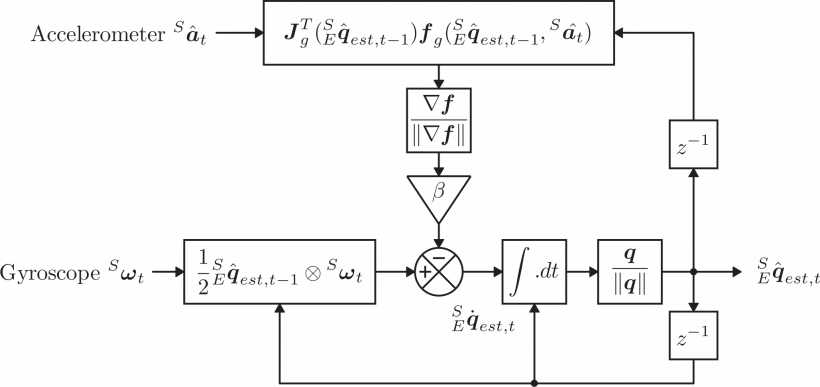
\includegraphics[width=1.0\textwidth]{figures/madgwick_imu.png}
    \caption{Block diagram representation of the orientation estimation algorithm.\cite{madgwick}}
    \label{fig:madgwick_imu}
\end{figure}

Implementations for various programming languages are available online\footnote{\url{https://x-io.co.uk/open-source-imu-and-ahrs-algorithms/}}, including an implementation for C. This C implementation was adopted for C++ and slightly modified. One of the modifications was the replacement of the ``fast inverse square-root'' by a more conventional implementation. The ``fast inverse square-root'' was producing biases and the computational performance was not too critical in our case anyway.

With an \gls{imu} based on accelerometer and gyroscope, the x and y-axis in world coordinates (see Figure \ref{fig:frames_of_reference}) will be rotated by an unknown angle around the z-axis. This is due to missing information of the horizontal orientation, which can only be observed by the magnetometer (in case of those three sensors). Moreover, this angle will be drifting due to accumulated errors coming from the gyroscope.

\section{Total rotation}

Since our hard iron calibration can only progress if the device is rotated, we might want to quantify the total rotation and use it instead of time as an axis for our prototyping and evaluation plots. This was achieved by calculating the Euler axis and angle between two orientation estimates and a sum over these angles.

The quaternion $\bm{\Delta q}_i$ that transforms the previous orientation $\bm{q}_{i-1}$ to the current orientation $\bm{q}_i$ can be expressed by the following equation.

\begin{equation}
\label{eq:impl_totalrot_q}
    \bm{q}_i = \bm{\Delta q}_i \times \bm{q}_{i-1} \iff \bm{\Delta q}_i = \bm{q}_i \times \bm{q}_{i-1}^{-1}
\end{equation}

The Euler angle can then be extracted with the extended Euler's formula.

\begin{equation}
\label{eq:impl_totalrot}
    \Delta \omega_i = 2 \arccos{\operatorname{Re}(\bm{\Delta q}_i)}
\end{equation}

With $\operatorname{Re}(\bm{\Delta q}_i)$ as the real component of the quaternion $\bm{\Delta q}_i$.

The summation over $\Delta \omega_i$ is our desired quantity ``total rotation''. This quantity was also used to filter for significant rotations in the filter routine of our hard iron calibration.

\section{Android}

Java was used to develop a small demo application that is able to read sensor data and pass it down to C++ through \gls{jni}. A webview was used to display the visualization written in JavaScript. The whole life cycle of the application was managed in Java.

The Android sensor \gls{api} offers a high-level interface to read sensor values by registering to a specific sensor type, like accelerometer, providing a sampling rate, and a callback for incoming data. The \gls{api} is presenting calibrated and uncalibrated sensor readings in the same way and is distinguishing between them by different identifiers. \textsc{TYPE\_MAGNETIC\_FIELD} can be used to read the system calibrated magnetic field and \textsc{TYPE\_MAGNETIC\_FIELD\_UNCALIBRATED} for the uncalibrated magnetic field, which is required by this thesis.\cite{android_sdk_sensormanager}

From experience we know that the sensor \gls{api} will not sample the sensors at a constant rate. Since a constant sampling rate is a requirement for the orientation filter, this problem had to be resolved as discussed in Section \ref{sec:impl_downsample}.

A screenshot of the demo application is shown in Figure \ref{fig:app}.

\begin{figure}[hbt!]
    \centering
    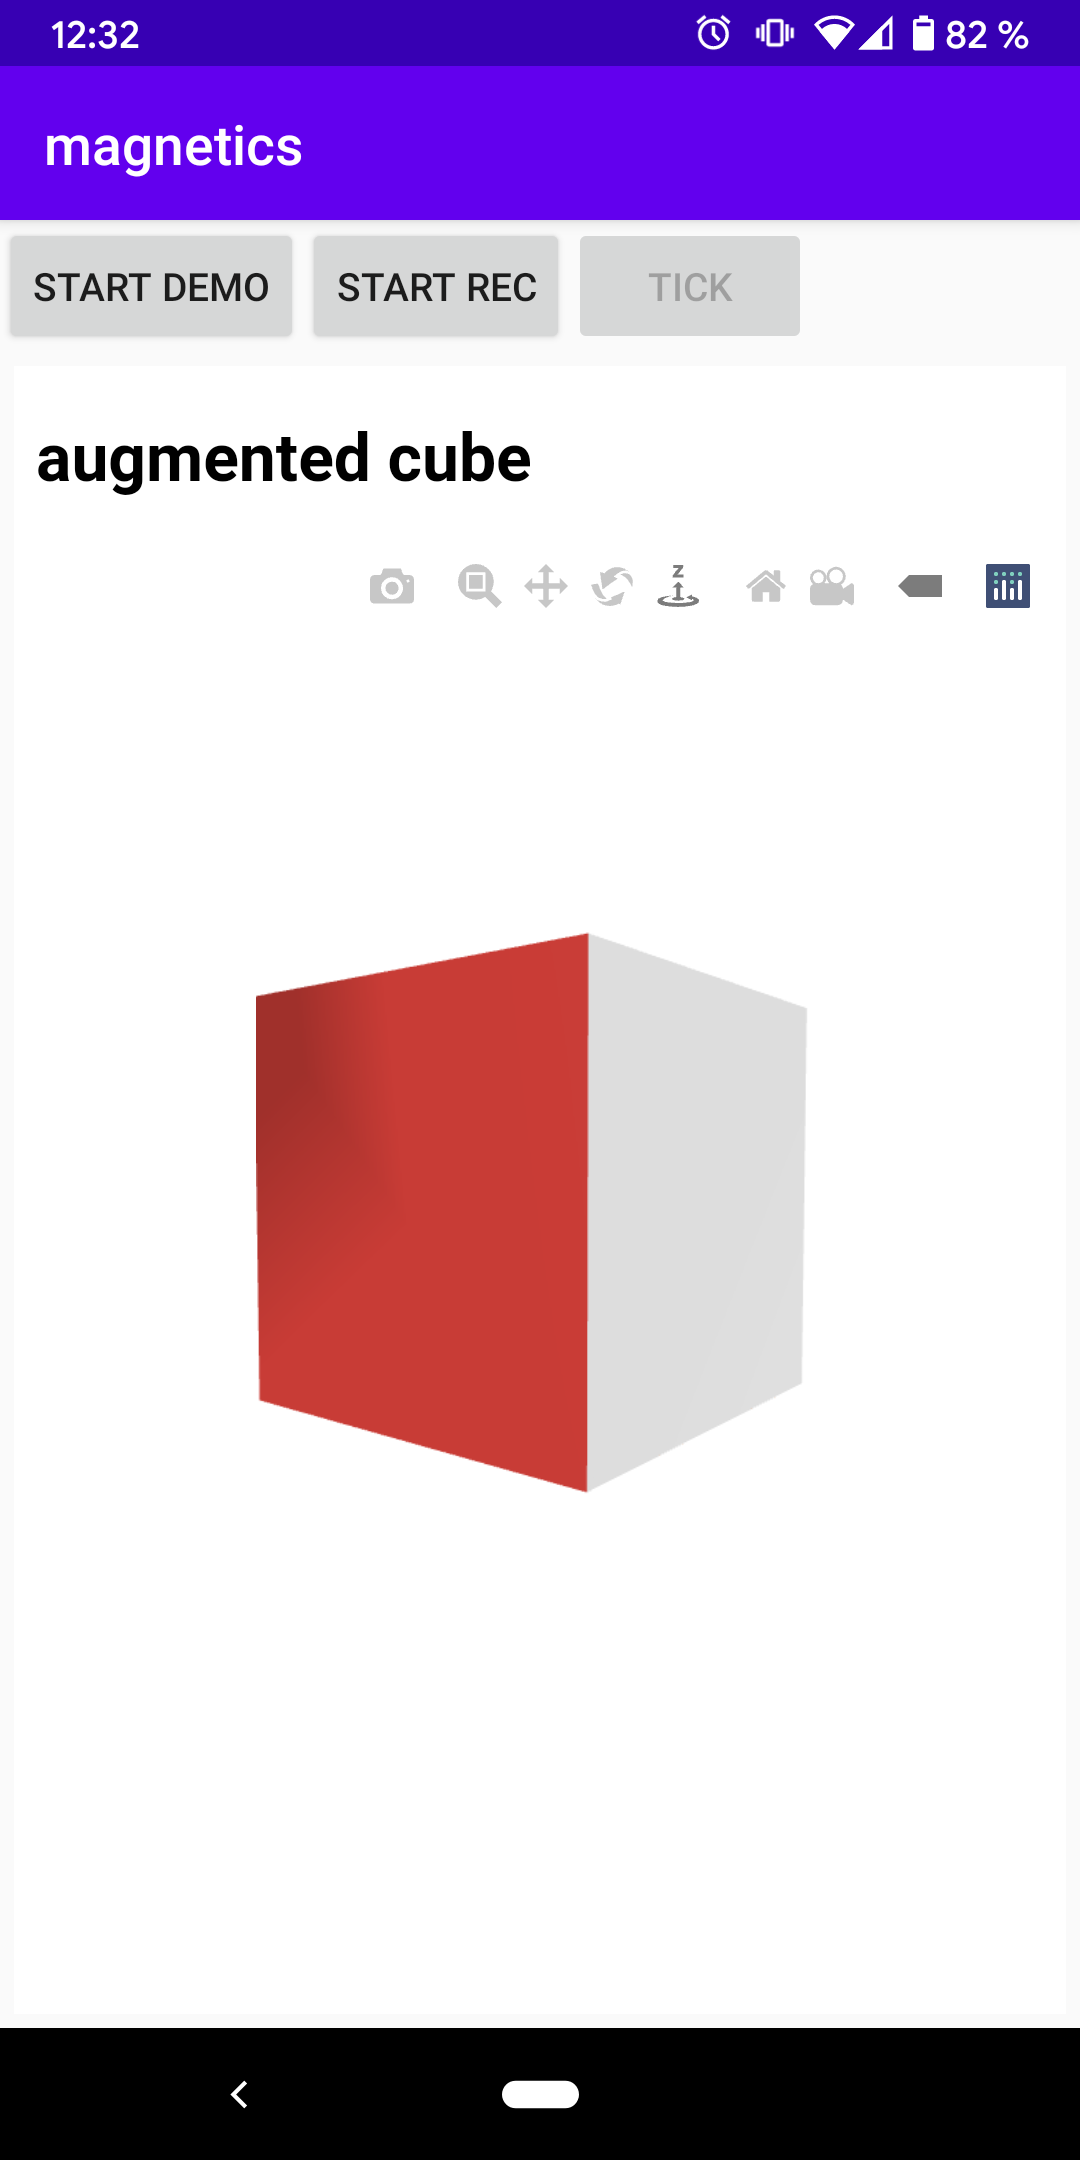
\includegraphics[width=0.4\textwidth]{figures/app.png}
    \caption{Screenshot for the Android demo application.}
    \label{fig:app}
\end{figure}

\section{Visualization}

One goal for the visualization was to build it platform independent use have the same code for desktop and mobile devices. This was beneficial because the visualization could also be driven by simulated and real-time sensor data.

% TODO dont tell the whole story. just state two options. then why one was preferred over the other
The initial idea was to use OpenGL ES for visualization purposes. Android and on common desktop \gls{os} support OpenGL. One visualization idea was a three-dimensional scatter plot for the acquired magnetic field sensor data to build up intuition for the data we are going to filter. This might require to plot thousands of data points in real time. Since OpenGL is executed by the \gls{gpu} there were no performance concerns.

Since implementation progress was rather slow and the effort was growing quickly the desire for an alternative was growing. JavaScript with plotly seemed to be a good solution for platform independence. It also claimed to have good performance with a WebGL backend for 3D plots.

The HTML and JavaScript code was stored as an asset along the demo application and was displayed with a webview on Android. On the desktop it is sufficient to use any modern browser to run the visualization.


\chapter{Empirical Evaluation}
\label{ch:eval}
% TODO section for explaining the evaluation process

In this chapter, we evaluate our implementation of the hard iron calibration presented in Chapter \ref{ch:impl}. First, we give an overview of the hardware used for evaluation. Then we take a look at the behaviour of the sensor data collection and a qualitative evaluation of the orientation filter. Finally, we will evaluate the quality of our hard iron calibration in comparison to the one of the system, the error estimation, and its performance.

\section{Hardware}

Four different devices were available for evaluation. They are listed in Table \ref{tbl:hardware}. It was important to compare the results between multiple devices since sensors and hard iron calibration algorithms vary between them. Also, we need to be sure that the performance of our implementation is good enough for real-time processing across different devices to achieve maximum compatibility.

All these devices run a fairly recent Android version and have been released during the last 5 years.

\begin{table}[h]
    \centering
    \begin{tabular}{ | l | r | r | }
    \hline
    \textbf{Name}     & \textbf{Release year} & \textbf{Android version} \\ \hline
    Google Pixel 3    & 2018 & 11 \\ \hline
    Google Pixel 2    & 2017 & 11 \\ \hline
    Samsung Galaxy S7 & 2016 & 8 \\ \hline
    LG Nexus 5X       & 2015 & 8.1 \\ \hline
    \end{tabular}
    \caption{Devices used for testing and evaluation.}
    \label{tbl:hardware}
\end{table}

Another possible test device was the Nokia 3 released in 2017 but unfortunately it does not provide uncalibrated magnetic field sensor readings. Up to this point we are not sure about the market share of devices that support uncalibrated readings. Alternatives will be discussed in Chapter \ref{ch:outlook}.

\section{Data collection}
\label{sec:eval_sensor}

The validation of the sensor data collection was a first and important step for evaluation, since all the following steps depend on it. Moreover, it was beneficial for building up intuition for the data which is used for filtering.

This experiment was carried out on all the Android test devices listed in Table \ref{tbl:hardware}. The requested sampling interval was $1$ ms.

As a first step, only the timestamps of the magnetometer readings were used to calculate the measurement interval. Since Android is not a real-time system the interval will not be constant. A histogram of the interval is shown in Figure \ref{fig:interval}. Statistics are given in Table \ref{tbl:mag_interval}.
% TODO point out that the measured sampling intervals is very different from the one requested

\begin{figure}[hbt!]
    \centering
    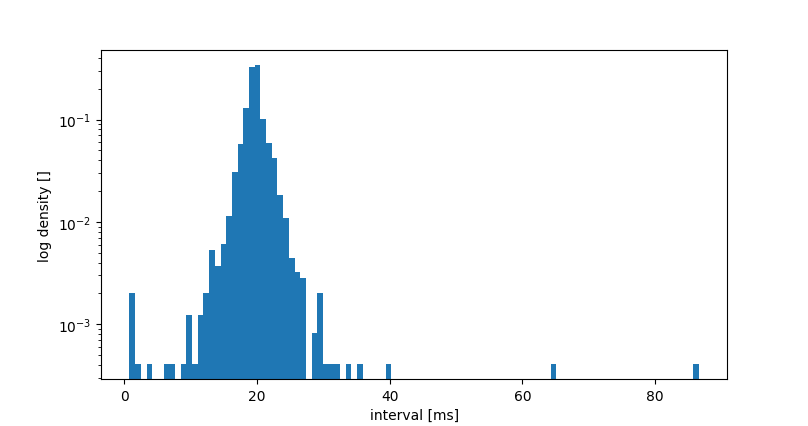
\includegraphics[width=1.0\textwidth]{figures/interval_nexus5.png}
    \caption{Histogram of the of the sampling interval for the magnetometer in the LG Nexus 5X.}
    \label{fig:interval}
\end{figure}

\begin{table}[h]
    \centering
    \begin{tabular}{ | l | r | r | r | r | r | r | r | }
    \hline
    \textbf{Device}   & \textbf{mean} & \textbf{std} & \textbf{min} & $\bm{Q_1}$ & \textbf{median} & $\bm{Q_3}$ & \textbf{max} \\ \hline
    Google Pixel 3    & 10.0 & 3.2 & 0.1 &  9.0 & 10.0 & 11.2 &  57.4 \\ \hline
    Google Pixel 2    &  9.6 & 1.6 & 0.0 &  9.2 &  9.6 &  9.9 &  63.9 \\ \hline
    Samsung Galaxy S7 & 10.0 & 2.6 & 0.3 &  9.3 & 10.0 & 10.7 & 115.5 \\ \hline
    LG Nexus 5X       & 19.7 & 2.6 & 0.8 & 19.0 & 19.7 & 20.4 &  86.5 \\ \hline
    \end{tabular}
    \caption{Statistics of the magnetometer reading interval in milliseconds.}
    \label{tbl:mag_interval}
\end{table}

Secondary, the readings of the magnetometer were displayed as a three-dimensional scatter plot to reveal the hard iron effect. For this purpose the device has been rotated in multiple directions while reading the magnetic field. Two-dimensional projections of such a three-dimensional scatter are shown in Figure \ref{fig:scatter} for the Samsung Galaxy S7.

\begin{figure}[hbt!]
    \centering
    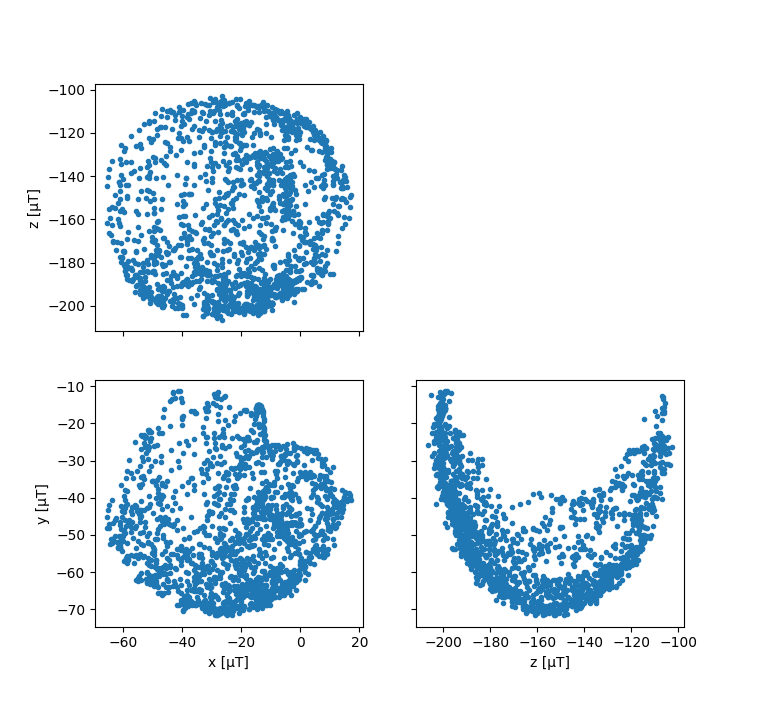
\includegraphics[width=1.0\textwidth]{figures/scatter_s7.png}
    \caption{Scatter plot of the magnetometer readings while rotating the Samsung Galaxy S7 in multiple directions.}
    \label{fig:scatter}
\end{figure}

Without the hard iron effect we would expect the center of the plots at the origin. The maximal distance from the origin should be the magnitude of the Earth's magnetic field if other environmental sources are neglectable. Measuring the horizontal orientation involves $\arctantwo(y, x)$ for a two dimensional projection of the magnetic field. As we can see in Figure \ref{fig:scatter}, without considering the hard iron effect, the estimation of the horizontal orientation would be meaningless since $(x, y, z)$ are not zero-centered.
% TODO there should be a sections for horizontal orientation estimation that we can reference here

\section{Orientation filter}
% TODO refer to impl section?

Since our hard iron calibration depends highly on the orientation estimation, it was necessary to validate the implementation and to evaluate its performance. A quantitative evaluation would require reference values for the orientation of the device for comparison. This could be achieved by tracking visual landmarks with a camera, rotating the device with a robotic arm or simulation of sensor data. Such experiments were carried out at the Department of Geodesy and Geoinformation at TU Wien in order to evaluate their Kalman-based orientation estimation.\cite{Ettlinger2018} However, using their equipment and data was not part of this thesis.

The implementation of the orientation filter required at least a qualitative evaluation to guarantee its functionality. This was carried out with an augmented reality demo application. A cube was placed at the origin of a 3D scene and the position and orientation of the camera in this scene were calculated based on the orientation of the phone in such a way, that the cube seems to be stationary in world coordinates. This approach validates the transformation between the local and global frames of reference and qualitatively evaluates the response to sensor updates.

The 3D scene is illustrated in Figure \ref{fig:cube_scene}. Pictures of the augmented cube rendered by the LG Nexus 5X are show in Figure \ref{fig:cubes}.

\begin{figure}[hbt!]
    \centering
    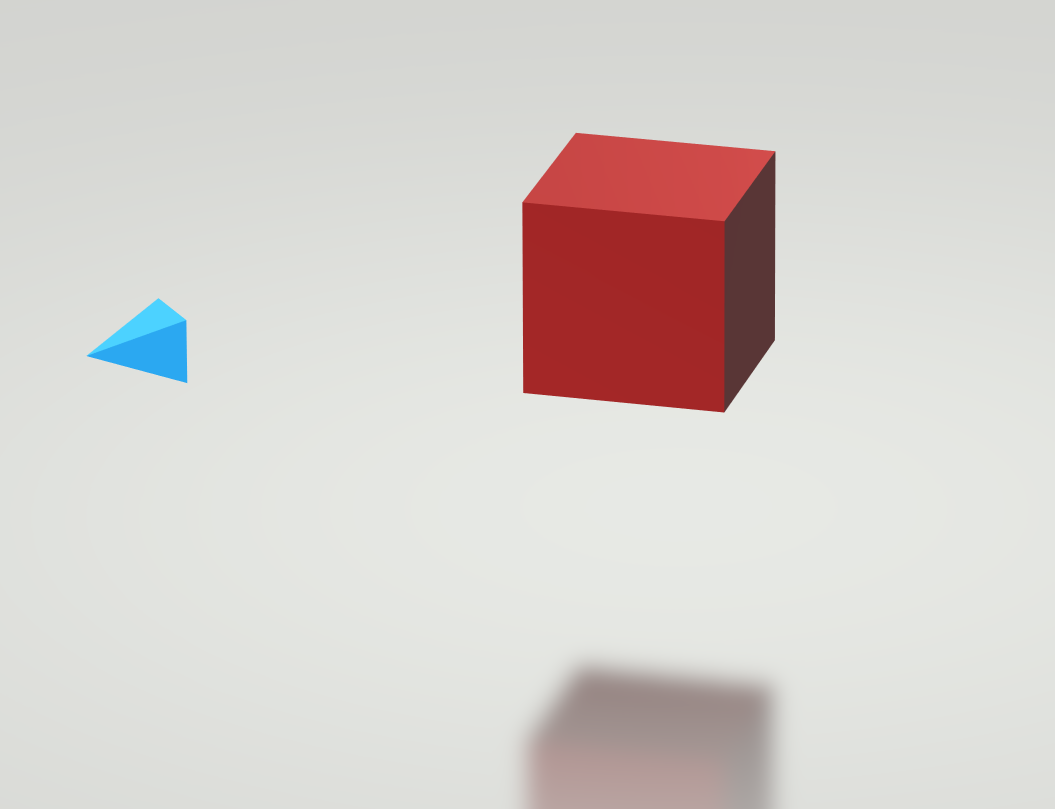
\includegraphics[width=0.6\textwidth]{figures/cube_scene.png}
    \caption{Illustration of the cube and the camera in the 3D scene.}
    \label{fig:cube_scene}
\end{figure}

\begin{figure}[hbt!]
    \centering
    \begin{subfigure}{0.3\textwidth}
        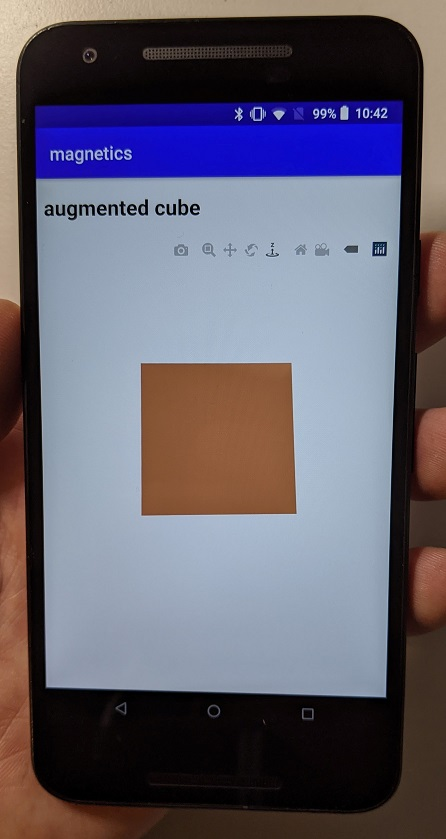
\includegraphics[height=1.5\linewidth]{figures/cube.jpg}
        %\caption{image1}
        %\label{fig:1}
    \end{subfigure}
    \begin{subfigure}{0.3\textwidth}
        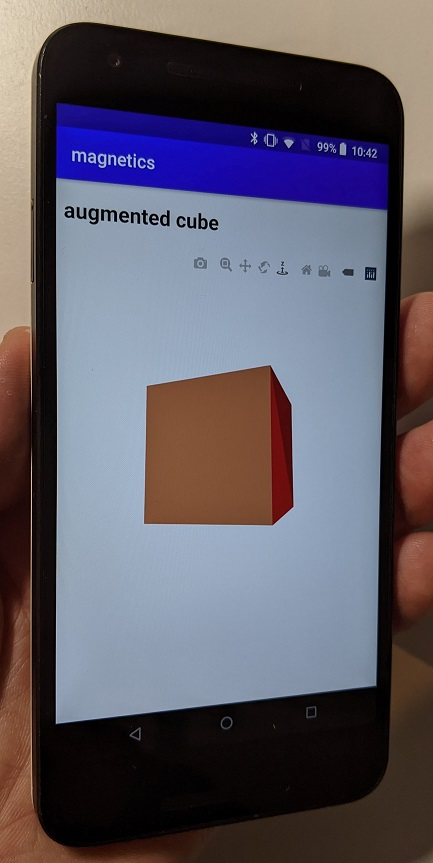
\includegraphics[height=1.5\linewidth]{figures/cube_right.jpg}
        %\caption{image1}
        %\label{fig:1}
    \end{subfigure}
    \begin{subfigure}{0.3\textwidth}
        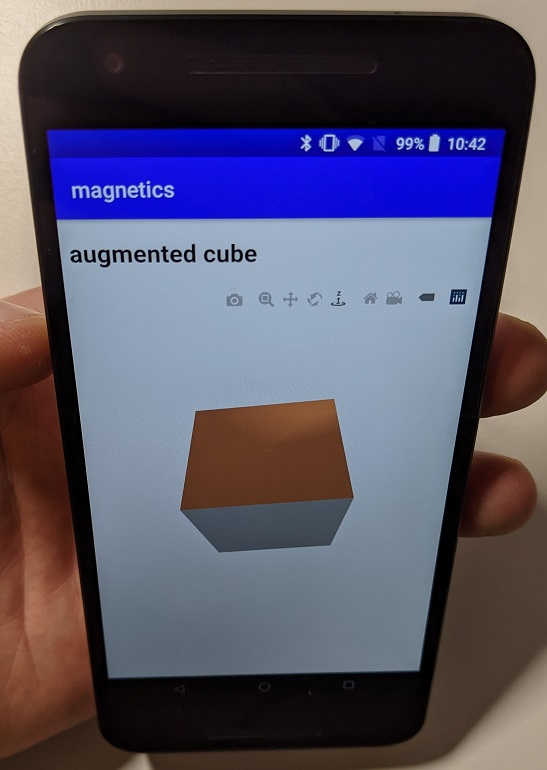
\includegraphics[height=1.5\linewidth]{figures/cube_bottom.jpg}
        %\caption{image1}
        %\label{fig:1}
    \end{subfigure}
    \caption{Pictures of the augmented cube after rotating the device.}
    \label{fig:cubes}
\end{figure}

The accelerometer and gyroscope have been down sampled to a 50 ms interval. Therefore, some delay and low refresh rate was expected. However, the experience was very positive.

The orientation filter has only a single parameter \textsc{beta}, apart from the update interval. \textsc{beta} models the reliability proportion between accelerometer and gyroscope measurements. This parameter has to be chosen carefully and in the best case individually for each sensor composition or smartphone model, since quality of the estimates depends highly upon that. Choosing one parameter across multiple devices might result in low accuracy or biased estimated.

Our demo application can be used to hand-tune \textsc{beta} for a given device. One could chose a parameter to start with and test it in the application. By observing the performance one might decide that the parameter is not optimal and change it. Following this process iteratively until the results are satisfying will lead to an optimized value for \textsc{beta}.

\section{Hard iron calibration}
% visualize particle cloud over time

% left over oscillations might be due to latency in orientation estimation or soft iron effects (read somewhere that magnetization only takes ns so that might be bs)
%  - rather small ~1µT so not that important for orientation but never the less interesting

A test track was set up in order to evaluate our hard iron calibration. It is illustrated in Figure \ref{fig:eval_scenario}. Visual landmarks were placed at each turning point as a spatial reference for the collected sensor data across different devices. The track had a total length of approximately 24 meters with 4 turns and a total horizontal rotation angle of approximately 540 degrees. A button in the test application, called \textsc{tick} (see Figure \ref{fig:app}), was used to mark the passing of each landmark.

\begin{figure}[H]
    \centering
    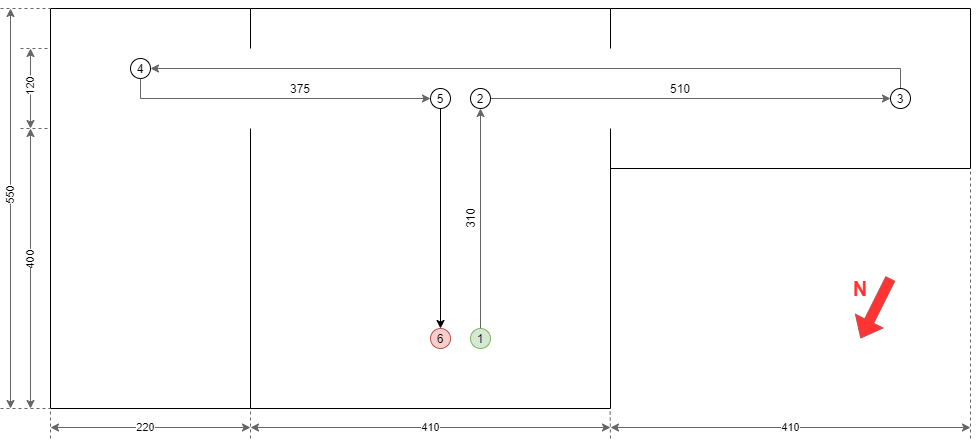
\includegraphics[width=1.0\textwidth]{figures/scenario.png}
    \caption{Illustration of the test scenario for the hard iron calibration.}
    \label{fig:eval_scenario}
\end{figure}

Each test run was a sequence of three different phases. In the first phase the test device was placed on a table. Thereby, the orientation estimation would initialize in the same way across different test runs. Then a magnet was used in order to manipulate the hard iron effect of the test device. The second phase started by pressing the \textsc{tick} button in the application, followed by walking the test track. The average walking speed was approximately 1 m/s. The third phase started with a last press of the \textsc{tick} button at landmark 6. Then the test device was rotated in multiple directions on the same position. With the third and last phase we collected a large amount of reference data for an optimal magnetometer calibration.

The test application would be started with the button \textsc{start rec} (see Figure \ref{fig:app}), an abbreviation for ``start recording''. By pressing this button, our application starts to record all the incoming data from the sensors. Our \textsc{tick} button is also treated like a sensor in this case. Each sensor reading is then stored in a file, along with its timestamp. The recorded data was later used to simulate the sensor input and to evaluate the output of our filter. Table \ref{tbl:eval_params} contains the parameters of our filter used during the simulation.

\begin{table}[H]
    \centering
    \begin{tabular}{ | l | r | }
    \hline
    \textbf{Parameter}              & \textbf{Value} \\ \hline
    \textsc{seed}                   & random \\ \hline
    \textsc{population}             & $10^5$ \\ \hline
    \textsc{deltaTime}              & 50 ms \\ \hline
    \textsc{initialVariance}        & $(100\ \mu T)^2$ \\ \hline
    \textsc{driftRate}              & $1.0$ \\ \hline
    \textsc{predictionVariance}     & $(5\ \mu T)^2$ \\ \hline
    \textsc{minimalRotation}        & $0.1$ \\ \hline
    \textsc{resamplingRate}         & $0.01$ \\ \hline
    \end{tabular}
    \caption{Chosen parameters for the simulation.}
    \label{tbl:eval_params}
\end{table}

The data of the third phase of our test runs was used to estimate an independent reference for the hard iron calibration. The chosen estimator was a least squares fit for a sphere with an unknown origin and radius.\cite{Jekel2016} 

Figures \ref{fig:eval_simulation_pixel3}, \ref{fig:eval_simulation_pixel2}, \ref{fig:eval_simulation_s7}, and \ref{fig:eval_simulation_nexus5x} show the \textcolor{blue}{estimated hard iron bias and error} of our particle filter over time compared to the \textcolor{red}{least squares} estimate. The vertical lines represent the time when a landmark was passed on the test track.

Tables \ref{tbl:eval_simulation_pixel3}, \ref{tbl:eval_simulation_pixel2}, \ref{tbl:eval_simulation_s7}, and \ref{tbl:eval_simulation_nexus5x} contain the values of the estimated hard iron bias and error across different methods after passing the landmarks on the test track. \textsc{PF} is our real-time particle filter estimate, \textsc{SYS} is the system's estimate, and \textsc{LS} the post processed least squares estimate. Phase 2.x denotes passing the landmark x on the test track. Phase 3 denotes the end of the experiment after rotating the phone in multiple directions.

In all our test cases the \gls{os} was not able to calibrate the hard iron effect while walking on the test track. Only in the last phase of the experiment, when the device was rotated in multiple directions. The estimates of the systems were very close to the least squares estimates.

Figure \ref{fig:eval_simulation_pixel3} and Table \ref{tbl:eval_simulation_pixel3} show the convergence of the hard iron estimation for the Google Pixel 3. Our particle filter calibration performed very well, but picked up a bias on the z-axis after landmark 4 (phase 2.4 in the table). During the calibration phase at the end of the experiment there was a bias on the x-axis.

\begin{figure}[H]
    \centering
    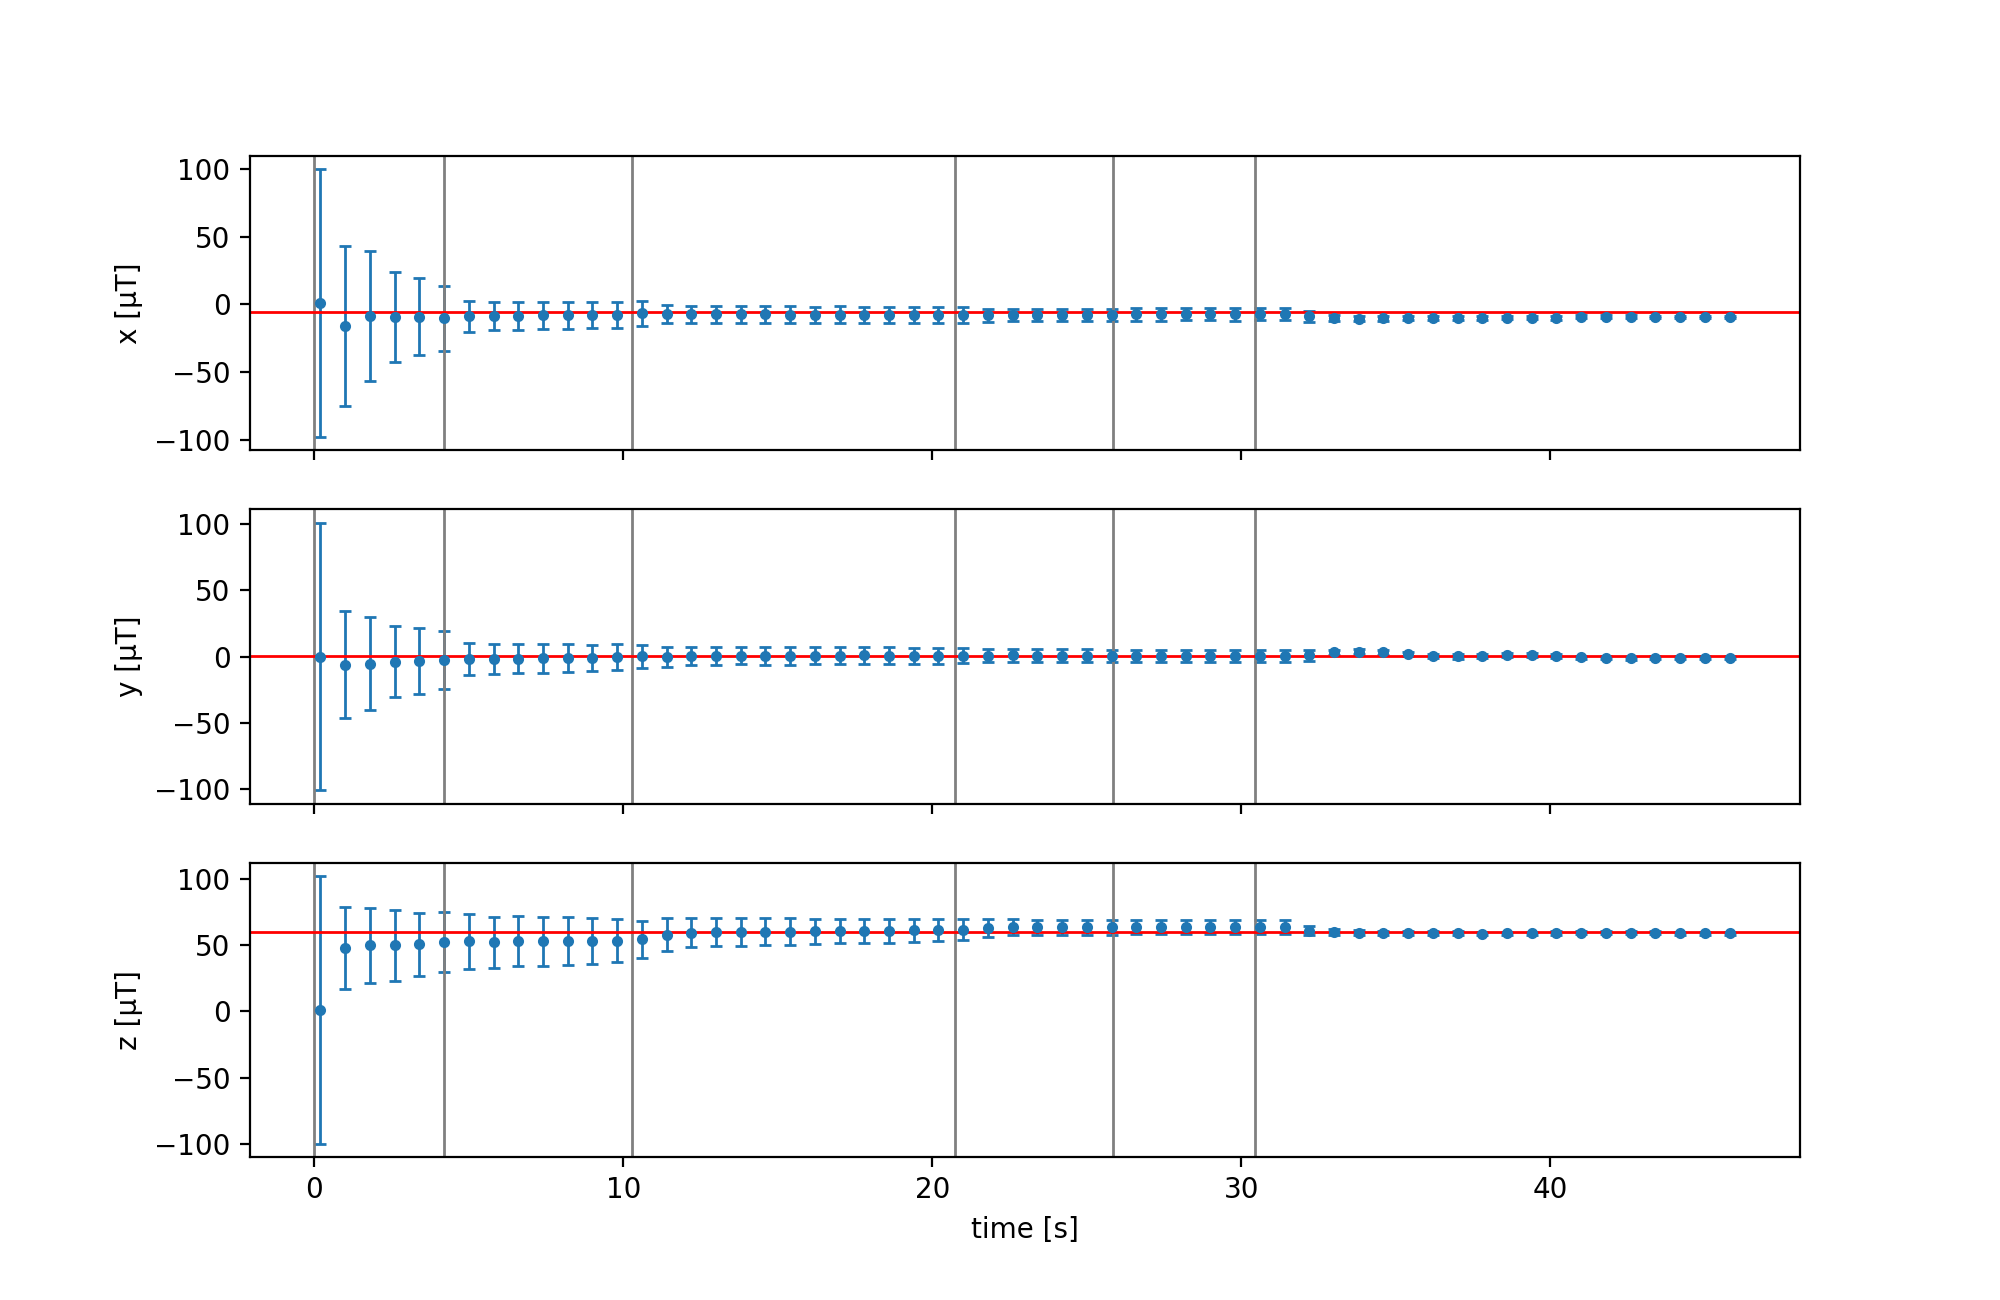
\includegraphics[width=1.0\textwidth]{figures/convergence_pixel3.png}
    \caption{Estimated hard iron bias and error over time on the Google Pixel 3.}
    \label{fig:eval_simulation_pixel3}
\end{figure}

\begin{table}[H]
    \centering
    \resizebox{\columnwidth}{!}{
    \begin{tabular}{ | l | l | r | r | r | r | r | r | r | }
    \hline
    \textbf{Method} & \textbf{Axis} & \textbf{Phase 2.1} & \textbf{Phase 2.2} & \textbf{Phase 2.3} & \textbf{Phase 2.4} & \textbf{Phase 2.5} & \textbf{Phase 2.6} & \textbf{Phase 3} \\ \hline
    PF  & X & $-0.5\pm100.5$ & $-9.3\pm24.0$ & $-5.8\pm7.2$ & $-5.3\pm4.6$ & $-5.3\pm3.9$ & $-4.9\pm3.7$ & $-8.4\pm1.1$ \\ \hline
    SYS &   & $1.0$ & $1.0$ & $1.0$ & $1.0$ & $1.0$ & $1.0$ & $-6.4$ \\ \hline
    LS  &   & & & & & & & $-5.4$ \\ \hline
    PF  & Y & $-0.6\pm100.4$ & $-3.7\pm21.6$ & $-3.3\pm8.8$ & $-2.4\pm5.0$ & $-2.3\pm4.1$ & $-2.4\pm4.0$ & $-0.9\pm1.1$ \\ \hline
    SYS &   & $32.6$ & $32.6$ & $32.6$ & $32.6$ & $32.6$ & $32.6$ & $1.3$ \\ \hline
    LS  &   & & & & & & & $0.3$ \\ \hline
    PF  & Z & $1.2\pm100.8$ & $52.1\pm22.5$ & $53.4\pm15.4$ & $61.5\pm8.1$ & $63.3\pm5.8$ & $63.7\pm5.4$ & $58.9\pm1.1$ \\ \hline
    SYS &   & $8.4$ & $8.4$ & $8.4$ & $8.4$ & $8.4$ & $8.4$ & $59.4$ \\ \hline
    LS  &   & & & & & & & $60.1$ \\ \hline
    \end{tabular}
    }
    \caption{Estimated hard iron bias in $\mu T$ with different methods on the Google Pixel 3.}
    \label{tbl:eval_simulation_pixel3}
\end{table}

Figure \ref{fig:eval_simulation_pixel2} and Table \ref{tbl:eval_simulation_pixel2} show the convergence of the hard iron estimation for the Google Pixel 2. Our particle filter calibration looks unbiased until landmark 6 (phase 2.6 in the table) but picked up a bias during the calibration phase at the end. Here we got a small bias for the x- and y-axis.

\begin{figure}[H]
    \centering
    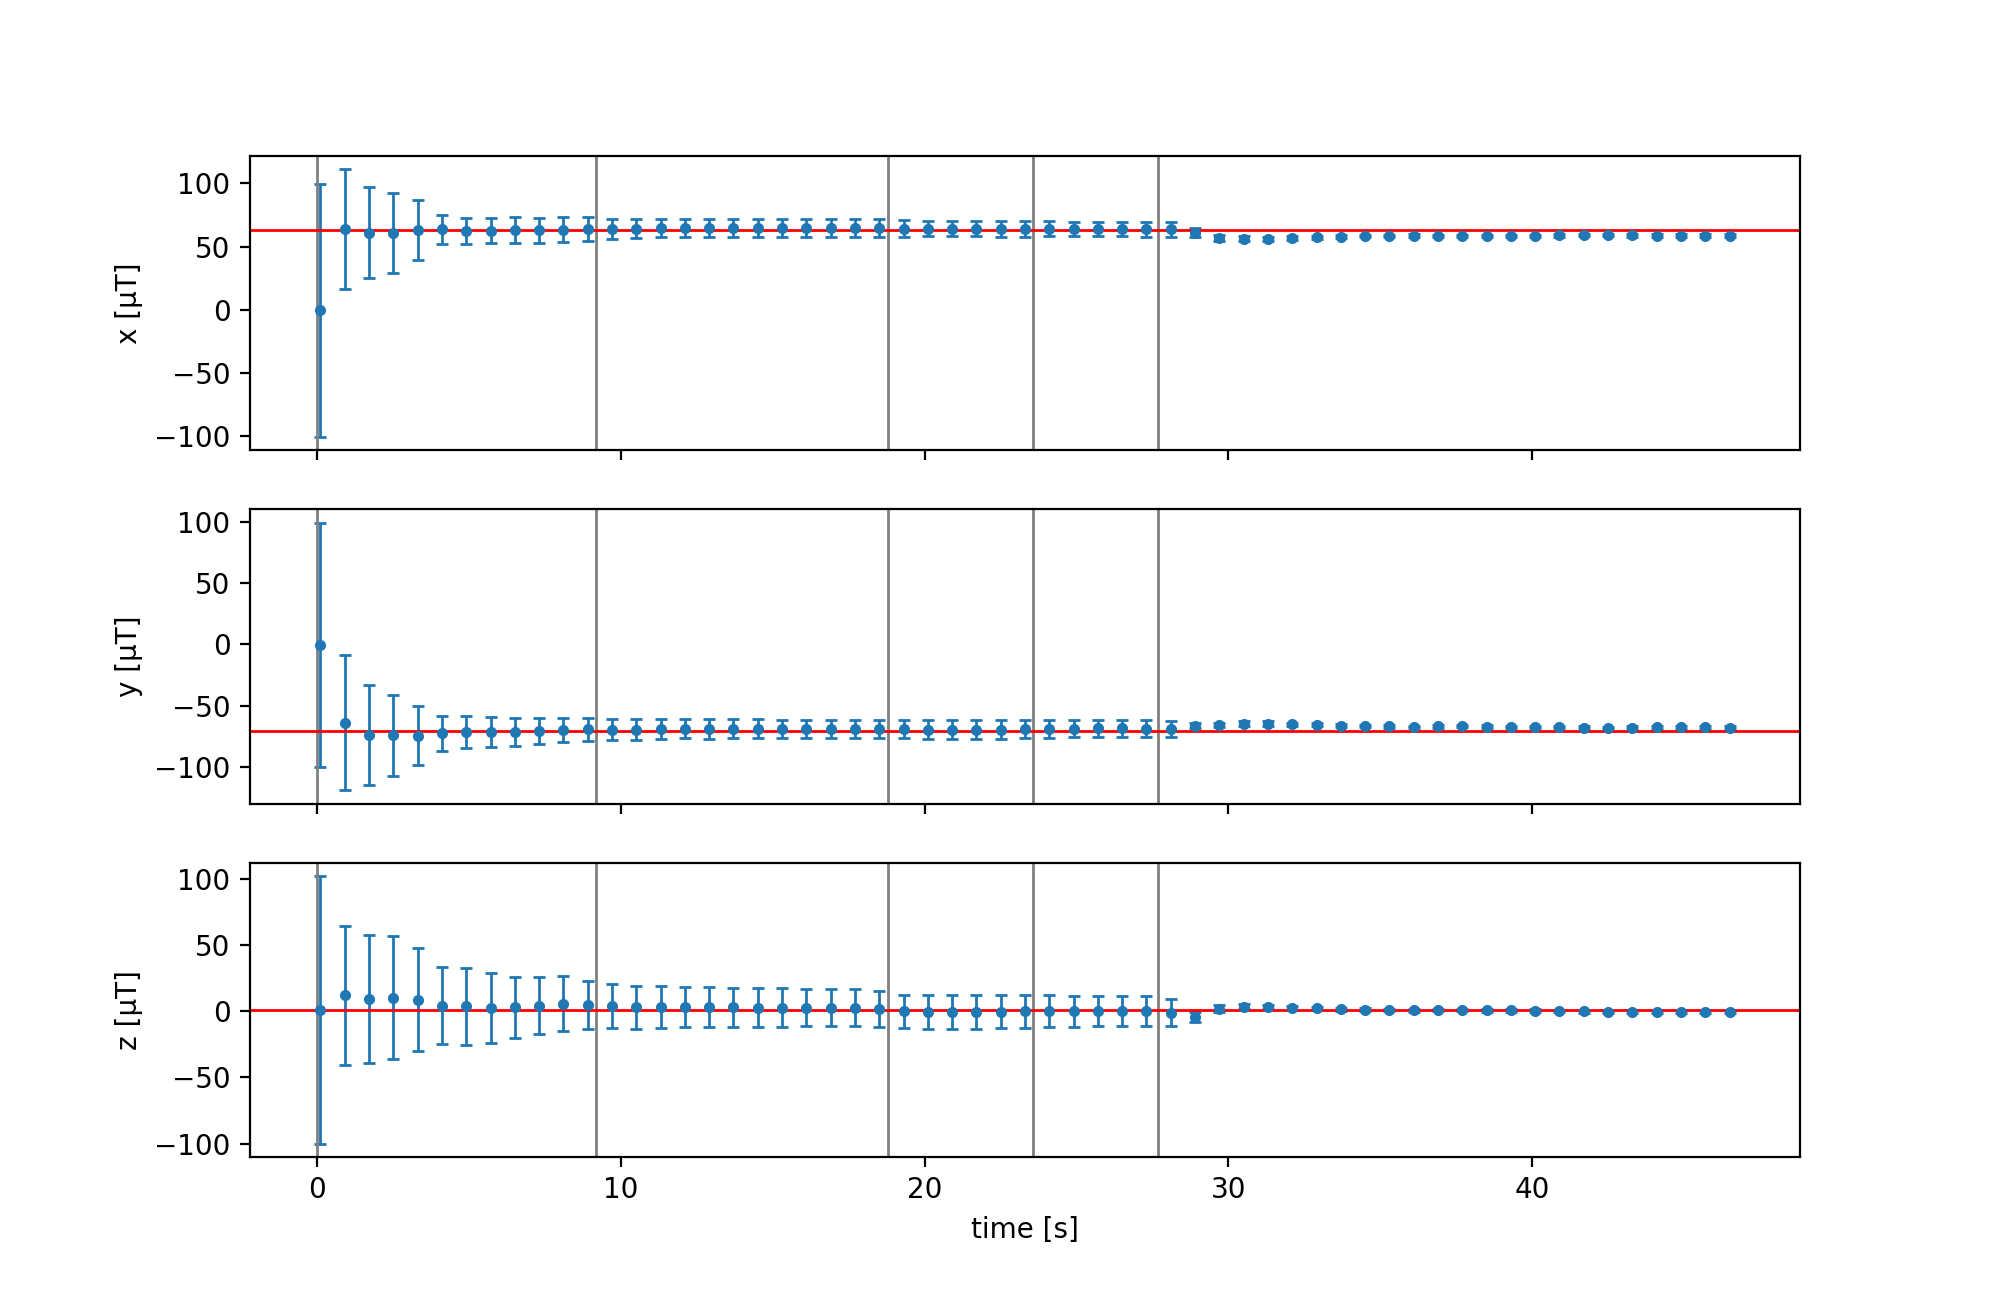
\includegraphics[width=1.0\textwidth]{figures/convergence_pixel2.png}
    \caption{Estimated hard iron bias and error over time on the Google Pixel 2.}
    \label{fig:eval_simulation_pixel2}
\end{figure}

\begin{table}[H]
    \centering
    \resizebox{\columnwidth}{!}{
    \begin{tabular}{ | l | l | r | r | r | r | r | r | r | }
    \hline
    \textbf{Method} & \textbf{Axis} & \textbf{Phase 2.1} & \textbf{Phase 2.2} & \textbf{Phase 2.3} & \textbf{Phase 2.4} & \textbf{Phase 2.5} & \textbf{Phase 2.6} & \textbf{Phase 3} \\ \hline
    PF  & X & $1.4\pm99.7$ & $62.3\pm9.1$ & $63.4\pm6.7$ & $62.7\pm5.1$ & $62.6\pm4.7$ & $59.8\pm1.7$ & $58.7\pm1.0$ \\ \hline
    SYS &   & $63.6$ & $63.6$ & $63.6$ & $63.6$ & $63.6$ & $63.6$ & $62.0$ \\ \hline
    LS  &   & & & & & & & $63.3$ \\ \hline
    PF  & Y & $0.9\pm100.1$ & $-68.7\pm11.4$ & $-70.0\pm7.6$ & $-69.1\pm6.2$ & $-68.8\pm5.8$ & $-64.2\pm1.9$ & $-67.9\pm1.0$ \\ \hline
    SYS &   & $-45.4$ & $-45.4$ & $-45.4$ & $-45.4$ & $-45.4$ & $-45.4$ & $-71.5$ \\ \hline
    LS  &   & & & & & & & $-71.2$ \\ \hline
    PF  & Z & $1.1\pm99.9$ & $1.4\pm17.7$ & $-1.2\pm11.7$ & $-0.5\pm9.2$ & $-0.0\pm8.2$ & $-3.1\pm1.6$ & $-0.2\pm1.0$ \\ \hline
    SYS &   & $-27.4$ & $-27.4$ & $-27.4$ & $-27.4$ & $-27.4$ & $-27.4$ & $-0.6$ \\ \hline
    LS  &   & & & & & & & $0.7$ \\ \hline
    \end{tabular}
    }
    \caption{Estimated hard iron bias in $\mu T$ with different methods on the Google Pixel 2.}
    \label{tbl:eval_simulation_pixel2}
\end{table}

Figure \ref{fig:eval_simulation_s7} and Table \ref{tbl:eval_simulation_s7} show the convergence of the hard iron estimation for the Samsung Galaxy S7. The hard iron effect of the z-axis was about 150 $\mu$T and therefore quite challenging. The filter would not initialize a lot of particles in close proximity since the \textsc{initialVariance} is just $(100\ \mu T)^2$. The y-axis picked up a bias most likely due to the same reason as the z-axis. During calibration phase the accuracy increases but a small bias remained on the x- and y-axis.

\begin{figure}[H]
    \centering
    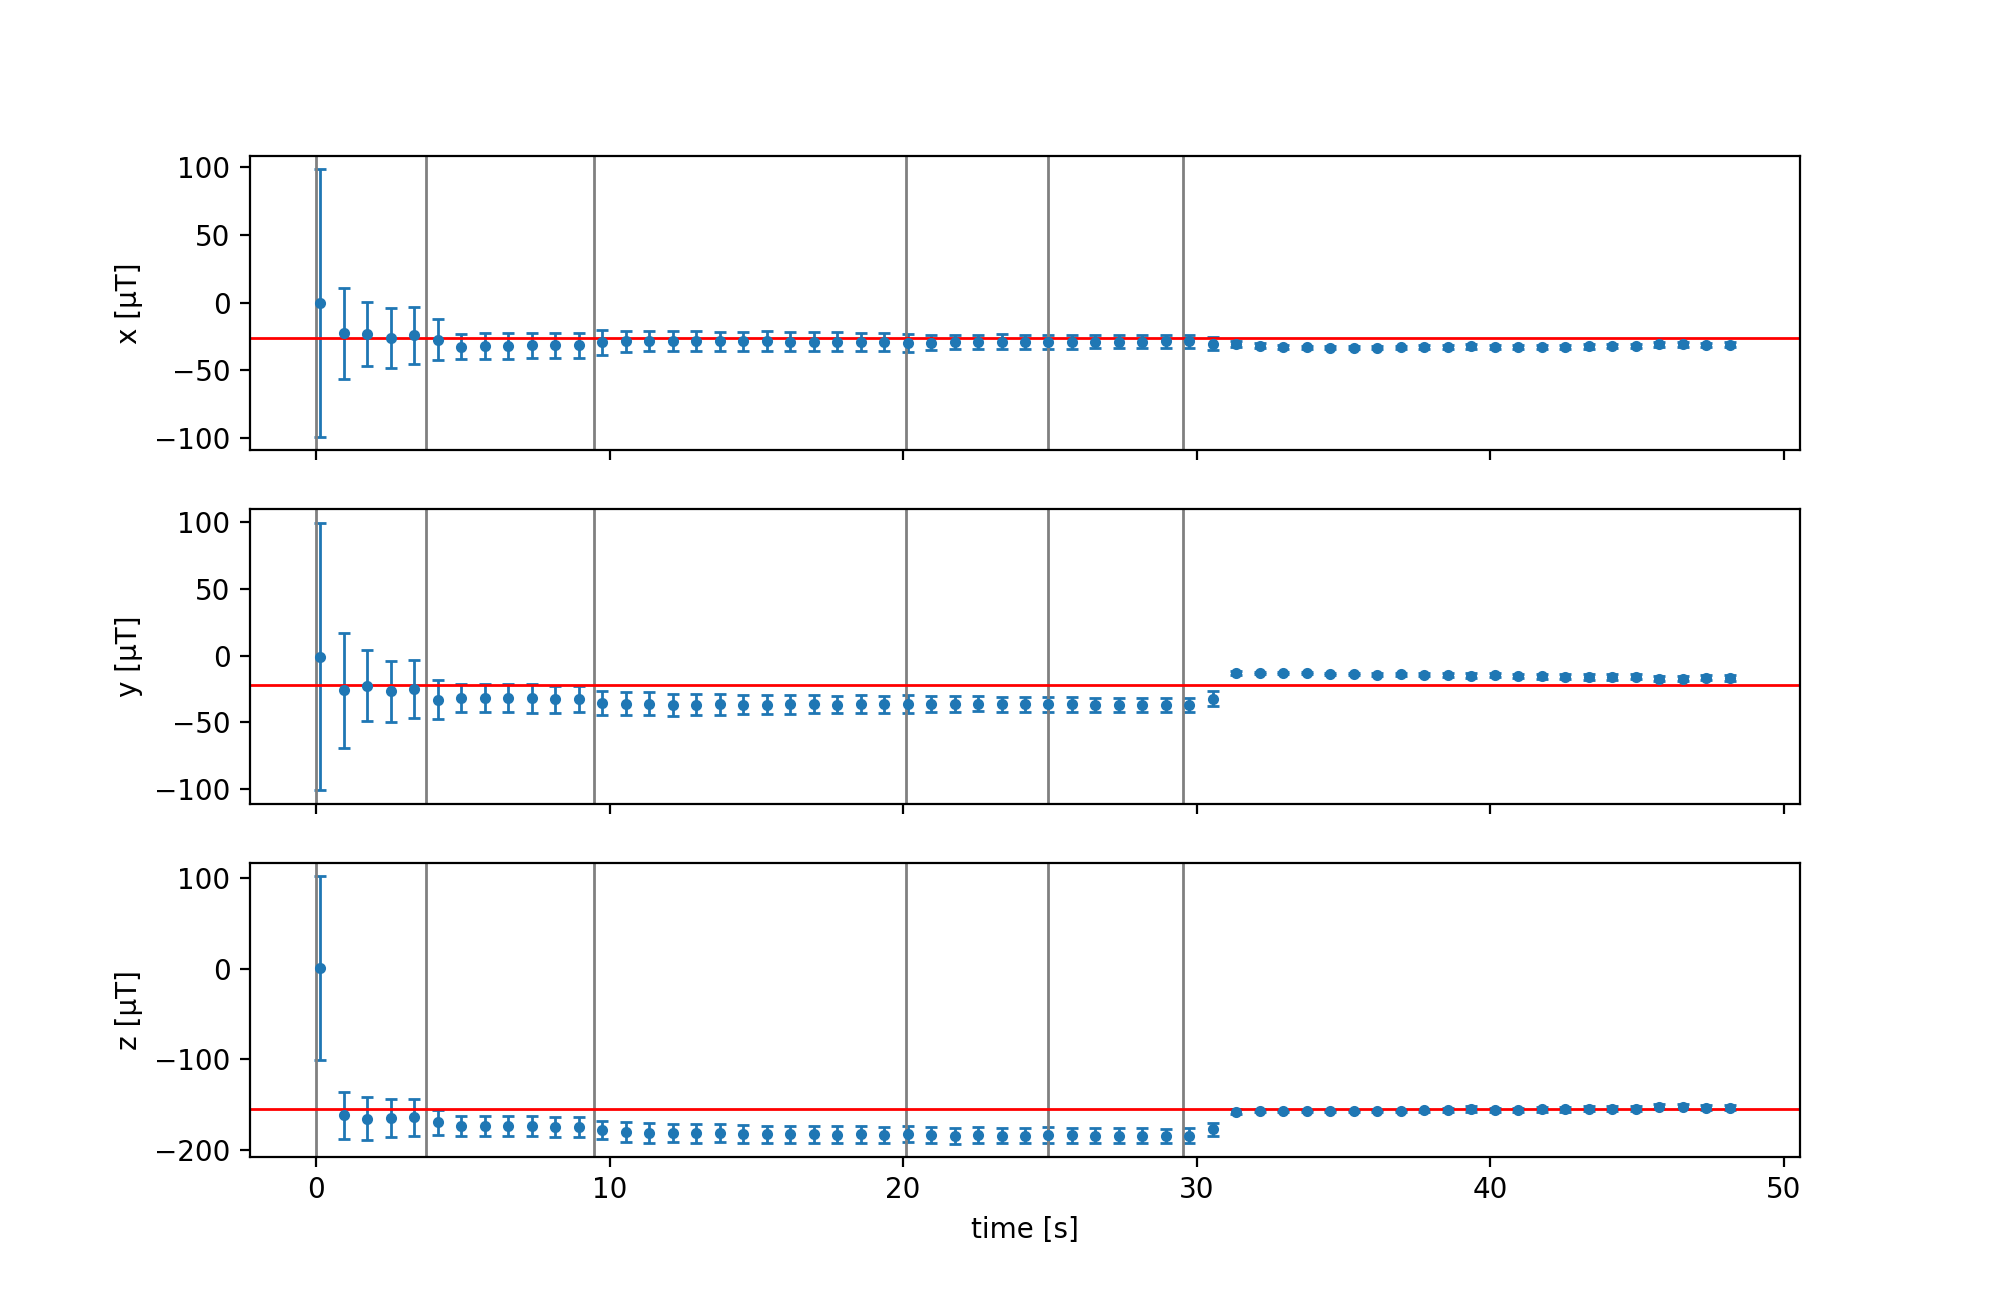
\includegraphics[width=1.0\textwidth]{figures/convergence_s7.png}
    \caption{Estimated hard iron bias and error over time on the Samsung Galaxy S7.}
    \label{fig:eval_simulation_s7}
\end{figure}

\begin{table}[H]
    \centering
    \resizebox{\columnwidth}{!}{
    \begin{tabular}{ | l | l | r | r | r | r | r | r | r | }
    \hline
    \textbf{Method} & \textbf{Axis} & \textbf{Phase 2.1} & \textbf{Phase 2.2} & \textbf{Phase 2.3} & \textbf{Phase 2.4} & \textbf{Phase 2.5} & \textbf{Phase 2.6} & \textbf{Phase 3} \\ \hline
    PF  & X & $1.1\pm100.0$ & $-20.9\pm17.2$ & $-24.1\pm7.0$ & $-24.9\pm5.5$ & $-25.8\pm4.4$ & $-26.1\pm4.2$ & $-27.2\pm1.1$ \\ \hline
    SYS &   & $0.0$ & $0.0$ & $0.0$ & $0.0$ & $0.0$ & $0.0$ & $-25.6$ \\ \hline
    LS  &   & & & & & & & $-26.1$ \\ \hline
    PF  & Y & $1.8\pm100.2$ & $-27.0\pm19.8$ & $-32.4\pm7.6$ & $-31.9\pm4.5$ & $-32.0\pm3.3$ & $-32.1\pm3.2$ & $-20.3\pm1.1$ \\ \hline
    SYS &   & $0.0$ & $0.0$ & $0.0$ & $0.0$ & $0.0$ & $0.0$ & $-23.6$ \\ \hline
    LS  &   & & & & & & & $-21.9$ \\ \hline
    PF  & Z & $0.9\pm99.9$ & $-163.8\pm16.7$ & $-167.7\pm8.9$ & $-169.8\pm6.4$ & $-170.7\pm5.1$ & $-171.1\pm4.9$ & $-154.9\pm1.2$ \\ \hline
    SYS &   & $0.0$ & $0.0$ & $0.0$ & $0.0$ & $0.0$ & $0.0$ & $-154.8$ \\ \hline
    LS  &   & & & & & & & $-154.6$ \\ \hline
    \end{tabular}
    }
    \caption{Estimated hard iron bias in $\mu T$ with different methods on the Samsung Galaxy S7.}
    \label{tbl:eval_simulation_s7}
\end{table}

Figure \ref{fig:eval_simulation_nexus5x} and Table \ref{tbl:eval_simulation_nexus5x} show the convergence of the hard iron estimation for the LG Nexus 5X. Our calibration performed reasonably well and remained within $\pm 1 \sigma$ until calibration phase. Our particle filter seemed to pick up oscillations from the rotations of the devices. This might be due to a bias in the orientation estimation. \textsc{beta} might not have been chosen optimal in this case.

\begin{figure}[H]
    \centering
    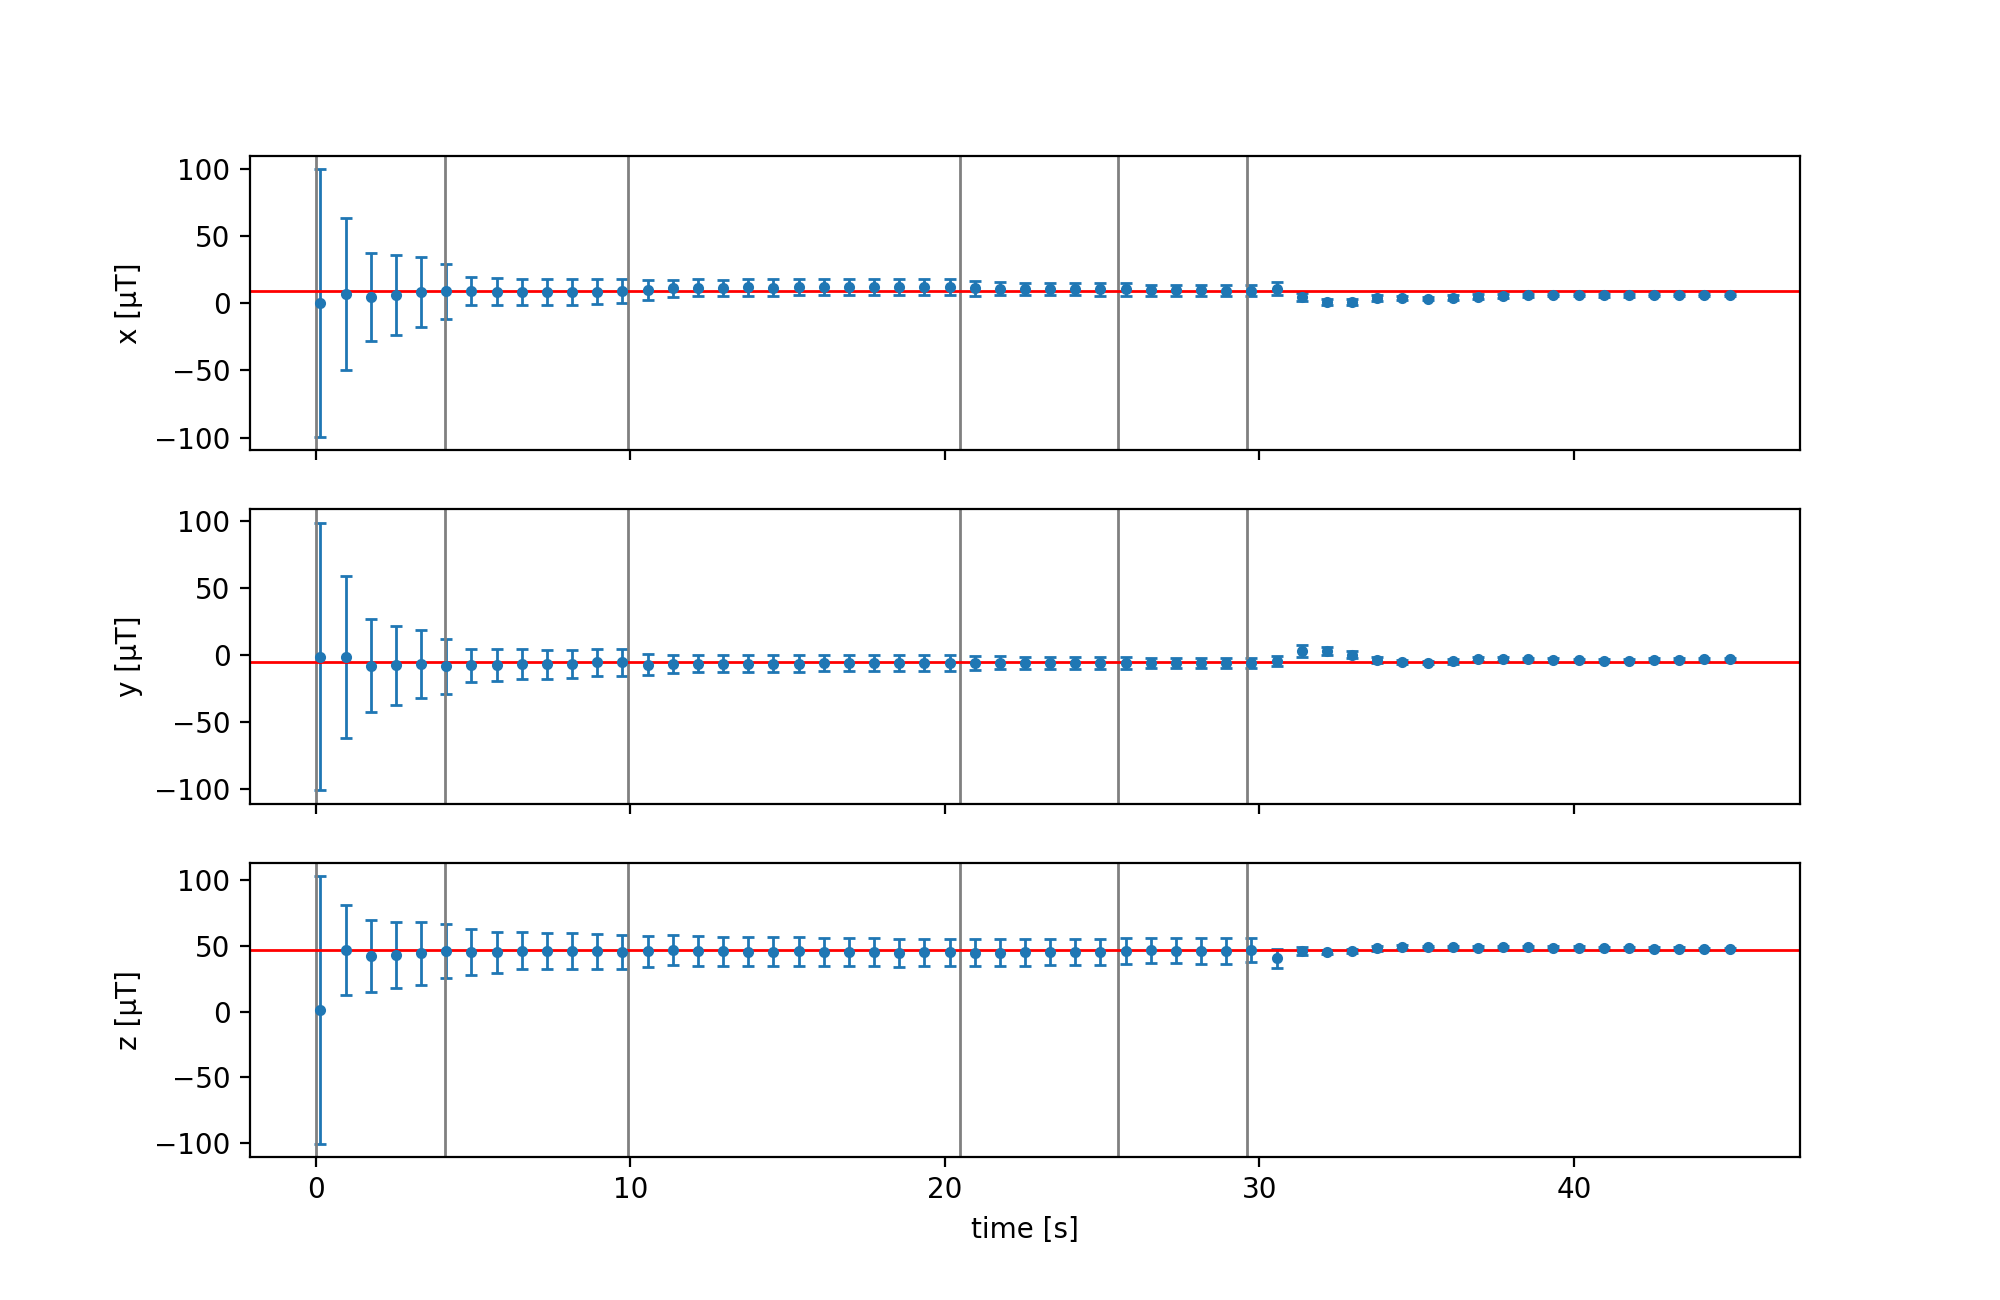
\includegraphics[width=1.0\textwidth]{figures/convergence_nexus5x.png}
    \caption{Estimated hard iron bias and error over time on the LG Nexus 5X.}
    \label{fig:eval_simulation_nexus5x}
\end{figure}

\begin{table}[H]
    \centering
    \resizebox{\columnwidth}{!}{
    \begin{tabular}{ | l | l | r | r | r | r | r | r | r | }
    \hline
    \textbf{Method} & \textbf{Axis} & \textbf{Phase 2.1} & \textbf{Phase 2.2} & \textbf{Phase 2.3} & \textbf{Phase 2.4} & \textbf{Phase 2.5} & \textbf{Phase 2.6} & \textbf{Phase 3} \\ \hline
    PF  & X & $0.4\pm99.4$ & $9.9\pm21.1$ & $7.1\pm9.6$ & $11.6\pm6.1$ & $11.3\pm4.4$ & $10.4\pm4.2$ & $2.9\pm1.1$ \\ \hline
    SYS &   & $-4.4$ & $-4.4$ & $-4.4$ & $-4.4$ & $-4.4$ & $-4.4$ & $10.6$ \\ \hline
    LS  &   & & & & & & & $9.2$ \\ \hline
    PF  & Y & $2.0\pm99.8$ & $-8.8\pm20.9$ & $-5.9\pm10.6$ & $-6.4\pm6.6$ & $-6.7\pm5.1$ & $-6.3\pm4.6$ & $-2.6\pm1.2$ \\ \hline
    SYS &   & $-47.8$ & $-47.8$ & $-47.8$ & $-47.8$ & $-47.8$ & $-47.8$ & $-6.7$ \\ \hline
    LS  &   & & & & & & & $-5.1$ \\ \hline
    PF  & Z & $-1.5\pm100.1$ & $45.9\pm20.7$ & $44.8\pm14.3$ & $40.6\pm10.3$ & $39.2\pm8.2$ & $39.8\pm7.7$ & $48.1\pm1.4$ \\ \hline
    SYS &   & $42.8$ & $42.8$ & $42.8$ & $42.8$ & $42.8$ & $42.8$ & $47.2$ \\ \hline
    LS  &   & & & & & & & $47.0$ \\ \hline
    \end{tabular}
    }
    \caption{Estimated hard iron bias in $\mu T$ with different methods on the LG Nexus 5X.}
    \label{tbl:eval_simulation_nexus5x}
\end{table}

In all our test cases the particle filter was able to converge. The estimated error dropped to approximately $\pm$ 6 $\mu$T after 20 seconds while producing biases of about $\pm$ 10 $\mu$T in the worst case. In phase 3, the accuracy of our filter was worse compared to the \gls{os} and least squares estimates. However, our particle filter produced results when the other methods were not able to. The biases might come from a previous signal processing step like the moving average or the orientation filter. Compared to the earth magnetic field the errors are reasonably small and should not affect the compass too dramatically.

\subsection{Computational performance}

Since we are targeting mobile devices and want to run our particle filter in real-time, the evaluation of the performance is indispensable. A fast algorithm has the benefit of being compatible with older and slower devices and will consume less battery which is a limited resource for mobile devices. Depending on the use case, the performance can be tweaked with the amount of particles. However, reducing the population of the particle filter will also reduce its stability. For a practical use case it is important to find a sweet spot with optimal performance and optimal stability.

The parameter \textsc{minimalRotation} was set to zero in order to measure an upper bound for the \gls{cpu} consumption. Otherwise the parameters were the same as shown in Table \ref{tbl:eval_params}.

The performance measurements are summarized in Table \ref{tbl:eval_performance}. Each value is the result of a 10 second measurement of the CPU time spent in the particle filter divided by real-time passed.

\begin{table}[h]
    \centering
    \begin{tabular}{ | l | r | r | r | r | r | }
    \hline
    \textbf{Device \textbackslash \ Population} & $10^3$ & $10^4$ & $10^5$ \\ \hline
    Google Pixel 3    & 0.00 & 0.06 & 0.51 \\ \hline
    Google Pixel 2    & 0.01 & 0.11 & 0.53  \\ \hline
    Samsung Galaxy S7 & 0.01 & 0.14 & 0.79  \\ \hline
    LG Nexus 5X       & 0.01 & 0.10 & 0.59  \\ \hline
    \end{tabular}
    \caption{CPU time spent in the particle filter divided by real-time passed per device and particle filter population.}
    \label{tbl:eval_performance}
\end{table}


\chapter{Conclusions}
\label{ch:conclusions}
The goal of this thesis was to overcome limitations of the \gls{os} hard iron calibration of smartphones in pedestrian navigation, localization and wayfinding scenarios, like \gls{ips} (more details in Section \ref{sec:ips}). We identified the following major limitations: different algorithms across different devices, dependence on gestures that have to be communicated to and performed by the user, no continuous calibration, and no quantified error estimation.

We proposed a particle filter to calibrate the hard iron effect of three-axis magnetometers in smartphones by sensor fusion with the accelerometer and gyroscope. Our algorithm can be updated iteratively and takes previous estimations into account. It does not depend on specific gestures that have to be communicated to the user. Any kind of rotations of the device are taken into account. Additionally, we can obtain a quantified error estimate for the hard iron calibration which can be used for error propagation in other filters that depend on the magnetic field (e.g. a compass).

A test plan was developed with a predefined track and different calibration phases to make the measurements of the different test devices comparable. We compared the results of the particle filter to those of the \gls{os} and to least squares estimates for reference. 

Our particle filter is producing promising results with a reasonable amount of CPU usage. It was able to calibrate the hard iron effect just by walking on the test track while the \gls{os} was not able to produce any estimates. This promotes our algorithm to a viable solution for online calibration of magnetometers in smartphones in navigation, localization and wayfinding scenarios. There is still a lot of room for improvements which are discussed in Chapter \ref{ch:outlook}.

As discovered during the work on this thesis, not all Android devices with a magnetometer will offer uncalibrated readings. Unfortunately, this limits the scope of application for our particle filter. Possible solutions are discussed in Chapter \ref{ch:outlook}.


\chapter{Outlook}
\label{ch:outlook}
% TODO kalman filter?
% TODO orientation error propagation

In this chapter we want to discuss possible future work connected to this thesis. Besides implementation details that might improve performance directly, there is room for further research on the model and applications.

In the evaluation our particle filter was biased in some cases. Depending on the application this need further investigation. Animating the time evolution of the state space might help to understand the underlying problem.

Currently the time evolution of the hard iron effect is modelled as a random walk. A possible improvement would be to have an adaptive speed for the random walk depending on the strength of the external magnetic field. More advanced models might even be able to predict the influence of the external field on the hard iron effect.

One application of this work is to develop an unbiased compass for smartphones in an indoor environment. Because of magnetic construction materials, the measured magnetic field can differ highly from the Earth's magnetic field. Since the variation of the building's magnetic field acts on much smaller scales than the one of the Earth, it might be possible to distinguish between them. Calibrating the hard iron effect is a preliminary step that removes one bias from the Equations \ref{eq:decomposition} and \ref{eq:decomposition_earth_env}. Simple models for the building's magnetic field might be that it is small compared to the Earth's field or that it is very chaotic and might chancel out in summation over a long path.

As discovered during the work on this thesis, not all Android devices with a magnetometer will offer ``uncalibrated'' readings, which do not contain hard iron compensation. Unfortunately, this limits the scope of application for our particle filter. This is true for at least the Nokia 3 and the Motorola Moto G3. Using the system's calibrated magnetometer readings for further calibrations requires caution, since it can be a new source of bias. It seems that the system calibration generates discontinuous jumps in the signal. It should be possible to filter these jumps and to propagate them into the state of the particle filter.

\section{Computational performance}

The particle filter is highly parallelizable because the particles are mostly independent. Only the resampling step usually requires interaction since a sum over all weights is performed.\cite{parallel_resampling}

Modern \glspl{cpu} come with special instructions for vectorization. Multiple operations, like vector addition, can be performed at the same time. This can speed up the execution time significantly if this happens on a critical path. Compiler Explorer\cite{compiler_explorer} can be used to check if such instructions are generated by the compiler.

Modern smartphones usually come with four processor cores or more. Those can be utilized by multithreading effectively. Usually that also requires synchronization which is error-prone and makes the program less readable.

Another possible optimization is to run the particle filter completely, or at least parts of it, on a \gls{gpu}. The \gls{gpu} is made for parallel and independent workloads and seems to fit well for this situation.\cite{parallel_resampling}

Performance is also related to battery consumption which is a critical resource for mobile devices. Depending on the application it might not be affordable to run a particle filter which is computational heavy by design.


%\cleardoublepage
%\pagenumbering{roman}
%\setcounter{page}{1}

\listoffigures
\addcontentsline{toc}{chapter}{List of Figures}
\listoftables
\addcontentsline{toc}{chapter}{List of Tables}
\listofalgorithms
\addcontentsline{toc}{chapter}{List of Algorithms}

\printglossary[type=\acronymtype]
\addcontentsline{toc}{chapter}{Glossary}

\printbibliography

\end{document}
